\let\pgfsavedyear\year
\documentclass{ieeeaccess}
\usepackage{cite}
\usepackage{amsmath,amssymb,amsfonts,mathtools,bm}
\usepackage{graphicx}
\usepackage{textcomp}
\usepackage{subcaption}
\usepackage{booktabs}
\usepackage{multirow}
\usepackage{longtable}
\usepackage{array}
\usepackage{tabularx}
\usepackage{algorithm}
\usepackage{algpseudocode}
\let\year\pgfsavedyear
\usepackage{tikz}
\usetikzlibrary{arrows.meta,positioning,shapes.geometric,calc,fit,backgrounds}
\usepackage{float}
\usepackage{xcolor}
\usepackage{url}
\usepackage{enumitem}
\usepackage{setspace}
\usepackage{hyperref}

\hypersetup{
  colorlinks=true,
  linkcolor=blue,
  citecolor=blue,
  urlcolor=blue
}
\def\BibTeX{{\rm B\kern-.05em{\sc i\kern-.025em b}\kern-.08em
    T\kern-.1667em\lower.7ex\hbox{E}\kern-.125emX}}
\definecolor{accessblue}{RGB}{0,98,155}
\makeatletter
\def\ps@titlepage{%
  \def\@oddhead{\parbox[t]{\textwidth}{\mbox{}\\[-6.3mm]\mbox{}\nheaderfont\color{accessblue}\headName\hfill\headerlogo{\raisebox{-2pt}{\,}}\color{black}\vspace*{-1.5mm}\par\hrulefill}}
  \def\@evenhead{\parbox[t]{\textwidth}{\mbox{}\\[-6.3mm]\mbox{}\headerlogo\hfill\nheaderfont\color{accessblue}\headName{\raisebox{-2pt}{\,}}\color{black}\vspace*{-1.5mm}\par\hrulefill}}
  \def\@oddfoot{\raisebox{3pt}{%
    \hbox to 0pc{\hbox to \textwidth{\mbox{}\hfill{\footervolfont\@pubid}\hfill\mbox{}}}%
    \hbox to 0pc{\hbox to \textwidth{\mbox{}\hfill{\footerpagefont\thepage}}}%
    }}
  \def\@evenfoot{\raisebox{3pt}{%
    \hbox to 0pc{\hbox to \textwidth{{\footerpagefont\thepage}\hfill}\mbox{}}\hspace*{1.8pc}%
    \hspace*{-1.8pc}\hbox to 0pc{\hbox to \textwidth{\mbox{}\hfill{\footervolfont\@pubid}\hfill\mbox{}}}%
    }}
}
\def\ps@headings{%
  \def\@oddhead{\parbox[t]{\textwidth}{\mbox{}\\[-6.3mm]{\raisebox{-2pt}{\headerfont\rightmark}}\hfill\headerlogoall\mbox{}\vspace*{-1.5mm}\par\hrulefill}}
  \def\@evenhead{\parbox[t]{\textwidth}{\mbox{}\\[-6.3mm]\mbox{}\headerlogoall\hfill{\raisebox{-2pt}{\headerfont\leftmark}}\vspace*{-1.5mm}\par\hrulefill}}
  \def\@oddfoot{\raisebox{8pt}{%
    \hbox to 0pc{\hbox to \textwidth{\mbox{}\hfill{\footerpagefont\thepage}}}%
    }}
  \def\@evenfoot{\raisebox{8pt}{%
    \hbox to 0pc{\hbox to \textwidth{{\footerpagefont\thepage}\mbox{}\hfill}}\hspace*{1.8pc}%
    }}
}
% The class calls \ps@headings ONCE, immediately, right after \documentclass
% is processed (not deferred inside \maketitle), so \@oddfoot/\@evenfoot are
% already locked in with the old "VOLUME..." text before the redefinition
% above would ever run again. Set them directly here so the change actually
% takes effect on body pages.
\def\@oddfoot{\raisebox{8pt}{%
  \hbox to 0pc{\hbox to \textwidth{\mbox{}\hfill{\footerpagefont\thepage}}}%
  }}
\def\@evenfoot{\raisebox{8pt}{%
  \hbox to 0pc{\hbox to \textwidth{{\footerpagefont\thepage}\mbox{}\hfill}}\hspace*{1.8pc}%
  }}
\makeatother

\begin{document}
\history{Date of publication xxxx 00, 0000, date of current version xxxx 00, 0000.}
\doi{10.1109/ACCESS.2017.DOI}
\title{ChurnFlux: Measuring and Recovering Per-Query Tail Recall Under Dynamic Updates in Graph-Based Approximate Nearest Neighbor Search}

\author{\uppercase{Daksh Agarwal}\authorrefmark{1},
\uppercase{S. Sobitha Ahila}\authorrefmark{1}}

\address[1]{School of Computer Science and Engineering, Vellore Institute of
Technology (VIT) Chennai, Tamil Nadu, India (e-mail: daksh.agarwal2025@vitstudent.ac.in; sobithaahila.s@vit.ac.in)}

\markboth
{Agarwal \headeretal: ChurnFlux: Query-Adaptive Robustness for Graph-Based ANN Search Under Churn}
{Agarwal \headeretal: ChurnFlux: Query-Adaptive Robustness for Graph-Based ANN Search Under Churn}

\corresp{Corresponding author: S. Sobitha Ahila (e-mail: sobithaahila.s@vit.ac.in).}

\begin{abstract}
Graph-based Approximate Nearest Neighbor (ANN) indexes power modern vector databases supporting semantic search, Retrieval-Augmented Generation (RAG), and recommendation systems. Although Hierarchical Navigable Small World (HNSW) indexes provide high retrieval accuracy and low latency, continuous insertions and deletions gradually deteriorate graph connectivity. This graph churn causes query-specific retrieval failures that are concealed by aggregate metrics such as average Recall@$K$, making retrieval robustness difficult to assess in dynamic environments.

This paper proposes \textbf{ChurnFlux}, a lightweight query-adaptive framework that improves retrieval robustness in dynamic graph-based ANN indexes without modifying the index structure. First, we introduce \textbf{Dynamic Robustness-$\delta@K$}, a query-centric metric exposing tail failures overlooked by average recall. Second, an oracle-free instability predictor estimates retrieval reliability from answer-set overlap of two lightweight probe searches. Third, an adaptive recovery mechanism allocates extra search effort only to predicted-unstable queries.

We evaluate ChurnFlux on HNSW and IVF-PQ under controlled churn across three datasets at up to 1.18M vectors (SIFT-1M, GloVe-200, Fashion-MNIST) over 5--50\% churn with multiple seeds. Average recall masks a substantial tail of failures at million-vector scale; the predictor identifies at-risk queries with AUC 0.83--0.94; and adaptive recovery improves the p1 tail from 0.44 to 0.60 on HNSW and from 0.14 to 0.24 on IVF-PQ at matched average cost. ChurnFlux treats the index as a black box, operating entirely in the query path for easy integration into existing HNSW-based and IVF-PQ-based systems.
\end{abstract}

\begin{keywords}
Adaptive Query Processing, Approximate Nearest Neighbor Search, Dynamic Graph Updates, Hierarchical Navigable Small World (HNSW), Retrieval Robustness, Retrieval-Augmented Generation, Vector Databases
\end{keywords}

\titlepgskip=-15pt

\maketitle

\begin{table}[!t]
\centering
\caption{Frequently Used Abbreviations}
\label{tab:abbrev}
\small
\begin{tabular}{ll}
\toprule
Abbreviation & Meaning \\
\midrule
ANN & Approximate Nearest Neighbor \\
HNSW & Hierarchical Navigable Small World \\
NSG & Navigating Spreading-out Graph \\
RAG & Retrieval-Augmented Generation \\
DPR & Dense Passage Retrieval \\
PQ & Product Quantization \\
$DR_{\delta}@K$ & Dynamic Robustness-$\delta$ at $K$ \\
$ef$ & HNSW search exploration parameter \\
\bottomrule
\end{tabular}
\end{table}

\section{Introduction}
\label{sec:introduction}

\PARstart{A}{pproximate} Nearest Neighbor (ANN) search has evolved from classical spatial partitioning structures \cite{Bentley1975, Friedman1977, Arya1998, Indyk1998} into a fundamental building block of modern data-intensive systems that operate on high-dimensional vector representations \cite{Xiao2024, VectorSurvey2024}. The rapid advancement of deep learning and pre-trained language models, such as BERT \cite{Devlin2019}, Sentence-BERT \cite{Reimers2019}, Dense Passage Retrieval (DPR) \cite{Karpukhin2020}, ColBERT \cite{Khattab2020}, ColBERTv2 \cite{Santhanam2022}, and FiD \cite{Izacard2021}, has significantly increased reliance on vector embeddings across dense retrieval \cite{Chen2024} and open-domain question answering. Applications such as semantic search, Retrieval-Augmented Generation (RAG) \cite{Lewis2020, Lewis2020_52, Gao2023_50, Zhao2024_40, Zhao2024_51, RAGSurvey2024, Guo2024_27, Ahn2022Access}, recommendation systems, and enterprise knowledge management rely on rigorous benchmark suites \cite{Thakur2021, Muennighoff2023, Lin2021} to evaluate retrieval quality across zero-shot and heterogeneous domains.

Among the numerous ANN indexing techniques---including product quantization \cite{PQ2011, Matsui2018}, anisotropic vector quantization \cite{ScaNN2020, Guo2020_45}, inverted multi-indexes \cite{Babenko2015}, hardware-accelerated platforms \cite{FAISS2019}, non-metric space libraries \cite{Boytsov2013}, SIMD-accelerated lookup tables \cite{Andre2019}, residual quantization \cite{Liu2015}, and multi-codebook quantization methods like Additive Quantization \cite{Martinez2016} and LSQ++ \cite{Martinez2018}---graph-based approaches have consistently demonstrated superior search performance. In particular, the Hierarchical Navigable Small World (HNSW) graph \cite{Malkov2020} and Navigating Spreading-out Graph (NSG) \cite{NSG2019, Fu2023} provide effective balances between search accuracy and computational efficiency. Consequently, graph methods form the backbone of both disk-resident libraries \cite{DiskANN2020, MicrosoftDiskANN, FreshDiskANN2022} and enterprise vector databases \cite{HAKES2025}, including Milvus \cite{Milvus}, Qdrant \cite{Qdrant}, Weaviate \cite{Weaviate}, Pinecone \cite{Pinecone}, OpenSearch \cite{OpenSearch}, and Elasticsearch \cite{Elastic}.

Unlike static benchmark datasets commonly used in ANN evaluation \cite{ANNBenchmarks2020, ANNBenchmarks2022, Aumuller2020_46, Simhadri2023, Simhadri2024}, production vector databases continuously evolve as new documents are inserted, obsolete information is removed, and existing knowledge is updated \cite{Xu2023, FreshDiskANN2022}. These frequent modifications gradually alter the topology of the underlying graph index. Although modern graph indexes support incremental updates \cite{Xu2025, CleanNN2025}, repeated insertions and deletions progressively deteriorate graph connectivity, leading to what is referred to in this work as \emph{graph churn}.

Conventional evaluation methodologies primarily measure retrieval performance using aggregate metrics such as average Recall@$K$. While these metrics provide useful system-level summaries, recent critiques point out that aggregate measures conceal substantial query-level failures \cite{Robust2025}. In practice, average Recall@$K$ may remain nearly constant even though certain queries experience severe retrieval failures. Such failures are particularly problematic in knowledge-intensive AI applications where inaccurate retrieval directly degrades downstream reasoning.

To illustrate why this matters in practice, consider a RAG-backed enterprise search system \cite{Lewis2020, RAGSurvey2024} built on a continuously updated HNSW index. As documents are ingested and retired over time, graph churn does not degrade every query uniformly: most queries continue to be served with high fidelity, so the system-wide average Recall@$K$ reported on a monitoring dashboard remains stable. A minority of queries, however, land in regions of the graph where churn has disproportionately disrupted local connectivity, and these queries silently receive incomplete or irrelevant context, which the downstream language model then reasons over as if it were reliable. Because the aggregate metric hides this tail, operators have no query-time signal indicating which individual answers are untrustworthy. This gap between system-level and query-level reliability is the central problem ChurnFlux is designed to close: rather than waiting for an aggregate metric to drift, it estimates, at query time and without ground truth, whether the specific query in hand is at risk, and reacts accordingly.

To mitigate graph deterioration, current systems often rely on graph repair or periodic rebuilding. However, recent empirical analyses show that fixed-budget graph repairs often fall into an ``interpolated-baseline trap'' where operational costs outweigh accuracy recovery benefits \cite{Mandarapu2026}. Furthermore, related hardness estimation techniques show that answer-set variability can signal search difficulty \cite{Sheaf2026}.

Taken together, these observations expose a concrete gap in the literature. Index-side solutions to graph churn---incremental repair \cite{Xu2025, CleanNN2025}, partial reconstruction \cite{DiskANN2020, FreshDiskANN2022}, and budget-matched maintenance \cite{Mandarapu2026}---treat every query with the same post-update search configuration, and \cite{Mandarapu2026} shows that this uniform treatment can spend real operational cost without recovering commensurate accuracy. Query-side difficulty estimators such as SHEAF \cite{Sheaf2026} move in the right direction by scoring individual queries, but they are not tied to a churn-aware evaluation metric and stop short of prescribing what a system should \emph{do} once a query is flagged as difficult. No existing approach combines a query-level robustness metric, an oracle-free instability signal, and a corresponding recovery action into a single mechanism that operates without touching the index. Closing exactly this gap is the goal of the present work.

To this end, this paper proposes \textbf{ChurnFlux}, a lightweight query-adaptive framework for robust ANN retrieval under dynamic graph updates. The novelty of ChurnFlux is threefold: it is, to our knowledge, the first framework to (i) make query-level retrieval robustness under churn directly measurable rather than inferring it from aggregate recall, (ii) predict which individual queries are at risk using only information available at query time---no ground truth, no access to the pre-churn graph---and (iii) close the loop by routing exactly those at-risk queries, and no others, to a boosted search, so that the extra cost is paid only where it is needed. Rather than modifying the graph structure, ChurnFlux operates entirely during query execution: it first estimates query instability using answer-set overlap derived from two lightweight probe searches, and then, based on that estimate, allocates additional graph exploration only to the queries predicted to be vulnerable.

The principal contributions of this work are summarized as follows:
\begin{itemize}
  \item \textbf{A query-level robustness metric.} We introduce \textbf{Dynamic Robustness-$\delta@K$}, an evaluation metric that reports the fraction of queries meeting a recall threshold rather than a single averaged score, directly exposing the tail failures that aggregate Recall@$K$ conceals \cite{Robust2025}.
  \item \textbf{An oracle-free instability predictor.} We propose a query instability test based on the Jaccard overlap between two lightweight probe searches at different exploration budgets, extending the answer-set flux principle of \cite{Sheaf2026} to the specific setting of dynamic graph churn, without requiring ground-truth neighbours or access to the pre-churn graph.
  \item \textbf{An adaptive, index-untouched recovery mechanism.} We develop \textbf{ChurnFlux}, which couples the instability predictor to a query-time recovery action: only queries flagged as unstable receive a boosted search, so the added cost scales with the number of affected queries rather than with index size, in contrast to graph reconstruction and repair strategies \cite{Mandarapu2026}.
  \item \textbf{Empirical validation under controlled churn.} We evaluate ChurnFlux on dynamically updated HNSW indexes built from standard ANN benchmarks \cite{ANNBenchmarks2020, ANNBenchmarks2022}, quantifying its effect on $DR_{\delta}@K$, tail recall, and search overhead relative to fixed-budget baselines.
\end{itemize}
\section{Related Work}
\label{sec:related}
Approximate Nearest Neighbor (ANN) search has been extensively studied in literature \cite{Xiao2024, VectorSurvey2024}. Existing research can be broadly classified into four categories: (i) graph-based and quantization-based ANN indexing, (ii) dynamic vector indexing and database architectures, (iii) hashing and similarity search methods, and (iv) retrieval robustness and adaptive query processing.
\subsection{Graph-Based and Quantization-Based ANN Search}
Graph-based ANN methods have demonstrated superior retrieval accuracy and efficiency. Early spatial partitioning and locality-sensitive hashing methods \cite{Bentley1975, Friedman1977, Indyk1998} paved the way for proximity graphs. Among modern graph structures, HNSW \cite{Malkov2020} constructs a multi-layer proximity graph that enables efficient greedy traversal. Navigating Spreading-out Graph (NSG) \cite{NSG2019, Fu2023} optimizes graph search paths by reducing edge redundancy. For large-scale settings, DiskANN \cite{DiskANN2020, MicrosoftDiskANN} enables compressed graph search on secondary storage, while FAISS \cite{FAISS2019} leverages GPU parallelization.
Quantization methods compress vector representations to reduce memory footprint. Product Quantization (PQ) \cite{PQ2011, Matsui2018} decomposes vector spaces into orthogonal subspaces, while Anisotropic Vector Quantization \cite{ScaNN2020, Guo2020_45} optimizes loss functions specifically for inner product search. Additive Quantization \cite{Martinez2016}, LSQ++ \cite{Martinez2018}, and Residual Vector Quantization \cite{Liu2015} further improve quantization precision. Accelerated lookup implementations such as Quicker ADC \cite{Andre2019} utilize SIMD registers to speed up distance calculations. Inverted Multi-Index structures \cite{Babenko2015} extend inverted files to multi-dimensional quantization, while Non-Metric Space Libraries \cite{Boytsov2013} expand search to arbitrary distance functions. Standard benchmark tools \cite{ANNBenchmarks2020, ANNBenchmarks2022, Aumuller2020_46, Simhadri2023, Simhadri2024} routinely confirm the recall-latency superiority of graph methods over quantization baselines. These static-index comparisons, however, say nothing about how either family behaves once the underlying data starts to change---the question we turn to next.
\subsection{Hashing and Dynamic Vector Indexing}
Hashing methods offer a complementary route to compact search: they map high-dimensional vectors to binary codes rather than pruning a proximity graph. Comprehensive surveys by Wang et al. \cite{Wang2014, Wang2016} and by Cao et al. \cite{Cao2018Access} detail learning-to-hash and binary-hashing strategies, while Multi-Index Hashing \cite{Norouzi2012} provides fast exact searches in Hamming space; as with the quantization methods above, this line of work optimizes for static, one-shot indexing rather than continuous updates. Continuous updates are, however, the norm in production: modern vector databases process streaming insertions and deletions as a matter of course \cite{Xu2023, FreshDiskANN2022}. A recent wave of work targets this directly at the index level. IP-DiskANN \cite{Xu2025} and CleanNN \cite{CleanNN2025} propose full-dynamism mechanisms that apply in-place edits to a graph index without full reconstruction; ACRONYM \cite{Acronym2026} explores in-memory acceleration for dynamic vector updates; and NAVIS \cite{Navis2026} minimizes position-seeking overhead on SSD storage during concurrent search and update. Related extensions such as ACORN \cite{Patel2024}, Starling \cite{Wang2024}, and EMA \cite{EMA2026} combine dynamic updates with general attribute filtering. Cloud-native systems including HAKES \cite{HAKES2025}, Milvus \cite{Milvus}, Qdrant \cite{Qdrant}, Weaviate \cite{Weaviate}, Pinecone \cite{Pinecone}, OpenSearch \cite{OpenSearch}, and Elasticsearch \cite{Elastic} package these mechanisms for enterprise-scale deployment. Yet a recent matched-budget analysis by Mandarapu and Kunkunuru \cite{Mandarapu2026} shows that these index-side repair strategies can fail to recover their own operational cost in accuracy terms once the comparison is budget-controlled---a negative result that directly motivates looking beyond the index for a remedy, and is a key piece of evidence this paper builds on.
\subsection{Dense Retrieval and Robustness Evaluation}
The queries that ANN indexes serve increasingly originate from dense neural retrieval rather than hand-crafted features. Dual-encoder models such as Sentence-BERT \cite{Reimers2019} and DPR \cite{Karpukhin2020} map text into dense embedding spaces, while late-interaction frameworks like ColBERT \cite{Khattab2020} and ColBERTv2 \cite{Santhanam2022} preserve token-level interactions, and generative retrieval techniques such as FiD \cite{Izacard2021} combine passage retrieval with generative decoding \cite{Chen2024, Devlin2019}. Benchmarking frameworks including Pyserini \cite{Lin2021}, BEIR \cite{Thakur2021}, and MTEB \cite{Muennighoff2023} evaluate this family of methods, but---like the ANN benchmark suites discussed above---almost exclusively through average Recall@$K$ or similar aggregate scores. This is precisely the evaluation gap that Wang et al. \cite{Robust2025} identify: aggregate metrics can remain stable even as a subset of queries experiences severe, silent retrieval failure. The stakes of this gap are highest in RAG applications \cite{Lewis2020, Lewis2020_52, Gao2023_50, Zhao2024_40, Zhao2024_51, RAGSurvey2024, Guo2024_27}, where a tail retrieval failure is passed directly to a language model that has no way to know its context is incomplete.
\subsection{Adaptive Query Processing and Difficulty Estimation}
If aggregate metrics hide which queries are failing, the natural response is to estimate difficulty per query rather than per system. Zhao \cite{Sheaf2026} introduced SHEAF, showing that query difficulty can be self-profiled from answer-set flux across varying search configurations---the observation that a query's sensitivity to its own search budget is itself informative, without needing a ground-truth label. This is the most closely related idea to the present work, and ChurnFlux builds directly on it: where SHEAF profiles general query hardness, ChurnFlux narrows the same probe-agreement principle to the specific, time-varying setting of graph churn, and extends it from a diagnostic signal into a closed-loop mechanism that also decides, and executes, the recovery action for each flagged query.
\subsection{Comparison with Existing Methods}
Table~\ref{tab:comparison} summarizes the differences between representative graph-based ANN approaches and ChurnFlux.
\begin{table*}[t]
\centering
\caption{Comparison of Existing ANN Retrieval Approaches}
\label{tab:comparison}
\small
\begin{tabular}{lccccc}
\toprule
Method & Dynamic Updates & Adaptive Query & Graph Recon. & Robustness Metric & Recovery \\
\midrule
HNSW \cite{Malkov2020} & \checkmark & $\times$ & $\times$ & $\times$ & $\times$ \\
NSG \cite{NSG2019} & $\times$ & $\times$ & $\times$ & $\times$ & $\times$ \\
DiskANN \cite{DiskANN2020, MicrosoftDiskANN} & \checkmark & $\times$ & Partial & $\times$ & $\times$ \\
FreshDiskANN \cite{FreshDiskANN2022} & \checkmark & $\times$ & Partial & $\times$ & $\times$ \\
IP-DiskANN \cite{Xu2025} & \checkmark & $\times$ & Partial & $\times$ & $\times$ \\
CleanNN \cite{CleanNN2025} & \checkmark & $\times$ & In-place & $\times$ & $\times$ \\
\textbf{ChurnFlux} & \checkmark & \checkmark & $\times$ & \checkmark & \checkmark \\
\bottomrule
\end{tabular}
\end{table*}
Beyond the presence/absence of each capability, the table also reflects where each method spends its computational budget. DiskANN, FreshDiskANN, IP-DiskANN, and CleanNN all amortize update cost by touching a bounded region of the graph on every insertion or deletion, but this cost is paid unconditionally, regardless of whether any query will ever traverse the affected region. ChurnFlux instead defers its extra cost to query time and pays it only for the subset of queries the instability predictor flags, which is why it is the only method in the table with both a robustness metric and a recovery mechanism: the two are designed together, with the metric identifying exactly the failures the recovery step is meant to address.
\subsection{Summary and Research Gap}
Table~\ref{tab:comparison} exposes a consistent pattern across the surveyed literature: systems that support dynamic updates efficiently (HNSW, DiskANN, FreshDiskANN, IP-DiskANN, CleanNN) do so by focusing on \emph{index-side} mechanisms---in-place edits, partial reconstruction, or streaming ingestion---while treating every query with an identical, static search budget once the update completes. None of these systems ask whether a specific incoming query is actually affected by the churn that has occurred, and none expose a metric that would reveal this at the query level; robustness is assessed, if at all, through aggregate Recall@$K$, which \cite{Robust2025} shows to be insensitive to tail failures. Conversely, difficulty-estimation techniques such as SHEAF \cite{Sheaf2026} operate at the query level but were not designed for, or evaluated under, dynamic graph churn, and graph-repair analyses such as \cite{Mandarapu2026} operate at the index level and do not offer a per-query remedy. ChurnFlux is positioned at the intersection of these two lines of work: it adopts a query-level difficulty signal in the spirit of \cite{Sheaf2026}, but applies it specifically to the churn setting, and pairs it with a lightweight, index-untouched recovery action rather than a global repair. This combination---query-level detection, oracle-free estimation, and selective query-time recovery---is, to the best of our knowledge, absent from the reviewed literature and constitutes the specific gap this paper addresses.

\section{Proposed ChurnFlux Framework}
\label{sec:method}

This section presents the proposed \textit{ChurnFlux} framework, a lightweight
middleware designed to improve the robustness of Approximate Nearest Neighbour
(ANN) retrieval under continuously evolving vector collections. Rather than
modifying the internal graph construction or maintenance strategy of an ANN
index, ChurnFlux operates transparently above the existing index and
adaptively increases the search effort only for queries that are likely to be
affected by graph churn.

The framework continuously observes vector insertions and deletions,
maintains runtime churn statistics, predicts query instability using
lightweight probe searches, and selectively invokes adaptive recovery whenever
required. Consequently, the underlying ANN backend remains unchanged while
retrieval robustness is improved with only limited computational overhead.

Figure~\ref{fig:architecture} illustrates the overall architecture of the
proposed framework. Client applications interact with the ChurnFlux middleware
through a unified search interface. The middleware continuously monitors graph
updates, estimates the current churn level, predicts unstable queries, and
selectively performs adaptive recovery before forwarding requests to the
underlying ANN backend. The detailed query execution pipeline is formalized
in Algorithms~\ref{alg:predictor} and~\ref{alg:adaptive}, and the graph churn
process used to age the index during evaluation is formalized in
Algorithm~\ref{alg:churn}.

%%%%%%%%%%%%%%%%%%%%%%%%%%%%%%%%%%%%%%%%%%%%%%%%%%%%%%%%%%%%%%%%%%%%%%%%%%%%%%%%

\begin{figure*}[!t]
\centering
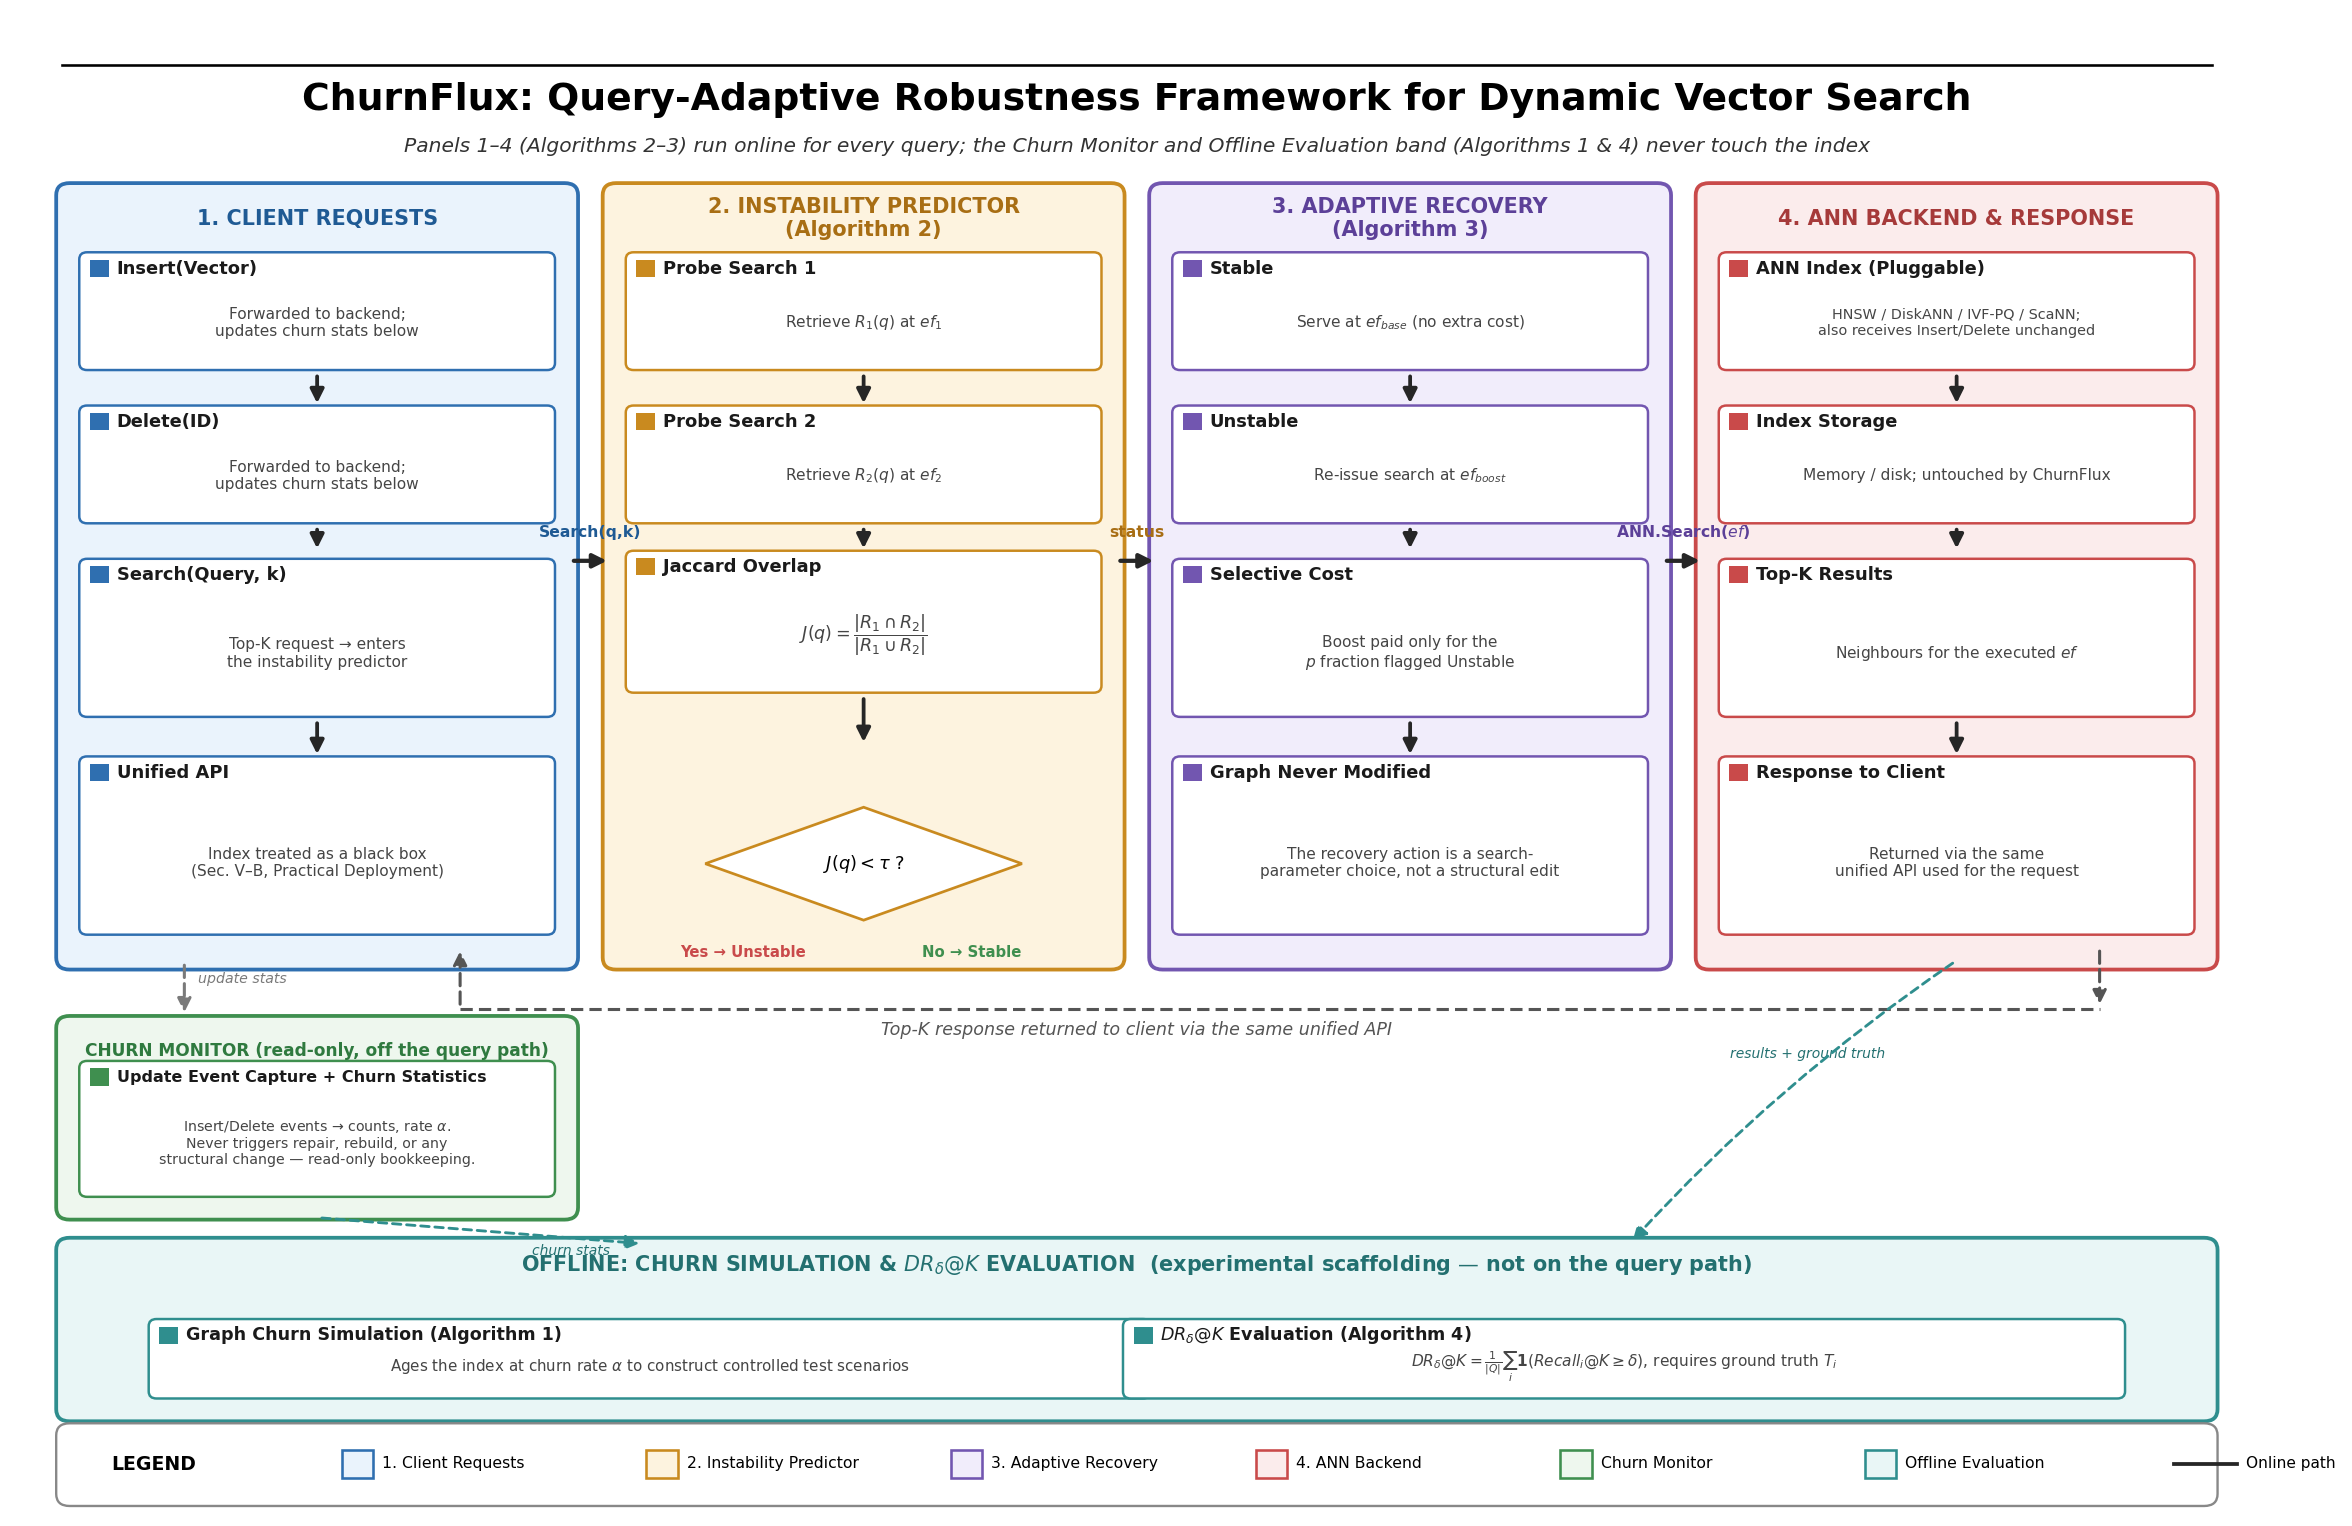
\includegraphics[width=\textwidth]{churnflux_architecture.png}
\caption{Client
applications issue search, insertion, and deletion requests through a unified
API. The ChurnFlux middleware monitors graph churn, estimates the current
churn level, predicts query instability using lightweight probe searches, and
selectively invokes adaptive recovery whenever necessary. The middleware
interfaces transparently with existing ANN backends (e.g., HNSW, DiskANN,
IVF-PQ, and ScaNN), enabling robust Top-$K$ retrieval without modifying the
underlying index implementation. Offline monitoring continuously evaluates
retrieval robustness using the proposed Dynamic Robustness-$\delta@K$
metric.}
\label{fig:architecture}
\end{figure*}


\subsection{Problem Formulation}
Let $V=\{v_1,v_2,\ldots,v_N\}$ denote a collection of $N$ vectors in $\mathbb{R}^{d}$. An HNSW index \cite{Malkov2020} is constructed as $G=(V,E)$. Under dynamic updates \cite{Xu2023, CleanNN2025}, at time $t$ the active graph is $G_t=(V_t,E_t)$. Given a query $q\in\mathbb{R}^{d}$, the goal is to retrieve Top-$K$ nearest neighbours $NN_K(q)$ robustly despite structural graph churn.

\subsection{Notation}
Table~\ref{tab:notation} summarizes the mathematical notation.

\begin{table}[!t]
\centering
\caption{Mathematical Notation}
\label{tab:notation}
\begin{tabular}{ll}
\toprule
Symbol & Description \\
\midrule
$G$ & Graph-based ANN index \\
$V$ & Vector collection \\
$E$ & Graph edges \\
$q$ & Query vector \\
$K$ & Number of retrieved neighbours \\
$ef$ & Search exploration parameter \\
$R$ & Retrieved neighbour set \\
$J$ & Jaccard overlap \\
$\tau$ & Instability threshold \\
$\delta$ & Robustness threshold \\
$DR_{\delta}@K$ & Dynamic Robustness metric \\
\bottomrule
\end{tabular}
\end{table}

\subsection{Dynamic Robustness-$\delta@K$}
Using the notation above, we first define the metric ChurnFlux is designed to improve, before turning to how it predicts and recovers instability at query time. Conventional Recall@$K = \frac{|R\cap T|}{|T|}$ averages performance across queries, hiding tail failures \cite{Robust2025}. We define Dynamic Robustness-$\delta@K$ as:
\begin{equation}
DR_{\delta}@K = \frac{1}{|Q|}\sum_{i=1}^{|Q|} \mathbf{1}\left(Recall_i@K \ge \delta\right),
\label{eq:dr}
\end{equation}
where $\delta\in[0,1]$ is the robustness threshold and $\mathbf{1}(\cdot)$ is the indicator function.

\subsection{Query Instability Prediction}
$DR_{\delta}@K$ measures robustness \emph{retrospectively}, over a query set for which ground truth is available. Deploying this idea at query time requires a signal that is available \emph{prospectively}, for a single query with no ground truth in hand---this is the role of the instability predictor introduced next. Following answer-set flux principles \cite{Sheaf2026}, ChurnFlux executes two probe searches with exploration budgets $ef_1$ and $ef_2$, producing sets $R_1(q)$ and $R_2(q)$. The Jaccard similarity is:
\begin{equation}
J(q)= \frac{|R_1(q)\cap R_2(q)|}{|R_1(q)\cup R_2(q)|}.
\label{eq:jaccard}
\end{equation}
Queries with $J(q) < \tau$ are classified as Unstable and routed to adaptive recovery. In practice, rather than fixing $\tau$ a priori, we calibrate it per workload as a percentile of the instability distribution observed during a brief warm-up phase, so that a target fraction of queries (the top 20\% most unstable) is routed to the boosted search. This makes ChurnFlux robust to dataset-specific overlap scales while keeping the decision rule simple and deployable: the threshold is a single workload-level configuration parameter, not a per-query choice.

\subsection{Design Rationale}
The instability predictor deliberately avoids any ground-truth signal, since exact neighbours are unavailable at query time in a production setting. Instead, it exploits a structural property of greedy graph search: at a low exploration budget ($ef_1$), the search terminates after visiting a small candidate frontier, so its output is highly sensitive to which edges local churn has added or removed. At a moderately larger budget ($ef_2$), the search explores a wider frontier and is more likely to converge on the same result regardless of small local perturbations. When $R_1(q)$ and $R_2(q)$ agree (high Jaccard overlap), the query sits in a well-connected, stable region of the graph and the cheap $ef_{base}$ search is already reliable. When they disagree (low overlap), the query lies near a decision boundary that churn has recently disturbed, and only then is the additional cost of $ef_{boost}$ justified. This design intentionally trades a small, bounded amount of duplicated search work (the second probe) for the ability to make this stable/unstable distinction without labels, oracles, or access to the pre-churn graph.

\subsection{Illustrative Example}
\label{sec:toyexample}
To make the instability test concrete, consider a toy example with $K=3$ and $\tau=0.65$ (independent of the experimental results in Section~\ref{sec:experiment}, shown here purely to illustrate the computation). Suppose a probe at $ef_1$ returns $R_1(q)=\{a,b,c\}$ and a probe at $ef_2$ returns $R_2(q)=\{a,b,d\}$ for the same query. Then $|R_1\cap R_2|=|\{a,b\}|=2$ and $|R_1\cup R_2|=|\{a,b,c,d\}|=4$, giving $J(q)=2/4=0.50$. Since $0.50<\tau$, this query is classified Unstable and re-executed at $ef_{boost}$. By contrast, if the two probes had returned identical sets, $R_1(q)=R_2(q)=\{a,b,c\}$, then $J(q)=3/3=1.0 \ge \tau$, and the query would be classified Stable, incurring no additional search cost. This example also shows why the test is oracle-free: computing $J(q)$ requires only the two probe results themselves, never the true neighbour set $T$.

\subsection{Algorithms}
With the metric, the predictor, and the recovery rule each motivated above, we now state all four as explicit algorithms and clarify how they fit together. Algorithm~\ref{alg:churn} formalizes the churn process used to age the index during evaluation: it is an \emph{offline} procedure, run between measurement rounds to simulate the effect of sustained insertions and deletions on the graph. Algorithm~\ref{alg:predictor} implements the query instability test defined by Eq.~\ref{eq:jaccard}, taking a query and the two probe budgets $ef_1, ef_2$ and returning a binary Stable/Unstable label; it is the only component that touches the index at query time beyond the search itself. Algorithm~\ref{alg:adaptive} wraps the predictor: it calls Algorithm~\ref{alg:predictor} once per query and uses its output to pick between the cheap baseline configuration $ef_{base}$ and the boosted configuration $ef_{boost}$, so that the extra cost of $ef_{boost}$ is paid only for queries the predictor flags. Algorithm~\ref{alg:robustness} is, like Algorithm~\ref{alg:churn}, an offline procedure: it takes the full query set together with ground-truth neighbours (available only during evaluation, not in production) and aggregates per-query outcomes into the $DR_{\delta}@K$ metric of Eq.~\ref{eq:dr}. In summary, Algorithms~\ref{alg:predictor}--\ref{alg:adaptive} constitute the online path executed for every query in production, while Algorithms~\ref{alg:churn} and \ref{alg:robustness} are experimental scaffolding used only to construct and evaluate the churn scenarios in Section~\ref{sec:experiment}.

\begin{algorithm}[!t]
\caption{Dynamic Graph Churn Simulation (offline, experimental)}
\label{alg:churn}
\begin{algorithmic}[1]
\Require Initial graph $G=(V,E)$ with $|V|=N$, churn rate $\alpha \in (0,1)$
\Ensure Updated graph $G_t$
\State Select $\alpha N$ active vertices uniformly at random
\State Mark selected vertices as deleted
\State Insert an equal number of replacement vectors \cite{Xu2023, CleanNN2025}
\State Update HNSW connectivity for affected regions \cite{Malkov2020}
\State \Return Updated graph $G_t$
\end{algorithmic}
\end{algorithm}

\begin{algorithm}[!t]
\caption{Oracle-Free Query Instability Prediction}
\label{alg:predictor}
\begin{algorithmic}[1]
\Require Query $q$, probe budgets $ef_1 < ef_2$, threshold $\tau$
\Ensure Stability label for $q$ (no ground truth used)
\State $R_1 \gets$ retrieve neighbour set using budget $ef_1$
\State $R_2 \gets$ retrieve neighbour set using budget $ef_2$
\State $J \gets \dfrac{|R_1\cap R_2|}{|R_1\cup R_2|}$
\If{$J<\tau$}
  \State \Return Unstable
\Else
  \State \Return Stable
\EndIf
\end{algorithmic}
\end{algorithm}

\begin{algorithm}[!t]
\caption{Adaptive Query-Time Recovery}
\label{alg:adaptive}
\begin{algorithmic}[1]
\Require Query $q$, budgets $ef_{base} < ef_{boost}$
\Ensure Top-$K$ neighbours for $q$
\State $status \gets$ output of Algorithm~\ref{alg:predictor} on $q$
\If{$status =$ Stable}
  \State Execute ANN search using $ef_{base}$
\Else
  \State Execute ANN search using $ef_{boost}$
\EndIf
\State \Return Top-$K$ neighbours
\end{algorithmic}
\end{algorithm}

\begin{algorithm}[!t]
\caption{Dynamic Robustness-$\delta@K$ Evaluation (offline, requires ground truth)}
\label{alg:robustness}
\begin{algorithmic}[1]
\Require Query set $Q$, ground-truth neighbours $T_i$ for each $q_i$, threshold $\delta$
\Ensure $DR_{\delta}@K \in [0,1]$
\State $count \gets 0$
\For{each query $q_i \in Q$}
  \State Compute $Recall_i@K = |R_i \cap T_i| / |T_i|$
  \If{$Recall_i@K \ge \delta$}
    \State $count \gets count + 1$
  \EndIf
\EndFor
\State $DR_{\delta}@K \gets count / |Q|$
\State \Return $DR_{\delta}@K$
\end{algorithmic}
\end{algorithm}

\subsection{Complexity and Overhead Analysis}
\label{sec:complexity}
The asymptotic cost of each ChurnFlux component is summarized as follows. The dominant online cost is the two probe searches, $O(ef_1 \log N)$ and $O(ef_2 \log N)$, plus the $O(K)$ Jaccard computation; for unstable queries an additional $O(ef_{boost}\log N)$ recovery search is incurred. Because $ef_1, ef_2 \ll ef_{boost}$ and, in the common case, most queries are classified Stable and never trigger the boosted search, the expected per-query overhead stays close to that of a single fixed-budget HNSW search. This is qualitatively different from graph-repair strategies, which must touch a substantial fraction of the index---incurring cost on the order of the repair scope, independent of whether a given query would have been affected---and which \cite{Mandarapu2026} show can fail to recover their own operational cost in accuracy terms. ChurnFlux instead spends its budget only where the instability predictor indicates it is needed, at the granularity of individual queries rather than the whole index. Insertion and deletion complexity is whatever the backend already provides ($O(\log N)$ for HNSW), plus a constant-time statistics update ($O(1)$); memory overhead is similarly limited to $O(N)$ for churn-monitoring metadata on top of the backend's own $O(NM)$ graph storage. Table~\ref{tab:complexity-body} summarizes this comparison against unmodified HNSW.

\begin{table*}[!t]
\renewcommand{\arraystretch}{1.2}
\caption{Computational complexity comparison between HNSW and the proposed ChurnFlux framework.}
\label{tab:complexity-body}
\centering
\begin{tabular}{lll}
\toprule
\textbf{Operation} & \textbf{HNSW} & \textbf{ChurnFlux} \\
\midrule
Search (Stable query) & $O(\log N)$ & $O(ef_1\log N)+O(ef_2\log N)+O(\log N)$ \\
Search (Unstable query) & $O(\log N)$ & as above $+\ O(ef_{boost}\log N)$ \\
Insertion & $O(\log N)$ & $O(\log N)+O(1)$ \\
Deletion & $O(\log N)$ & $O(\log N)+O(1)$ \\
Graph maintenance & Periodic rebuilding (optional) & Not required; index untouched \\
Memory & $O(NM)$ & $O(NM)+O(N)$ \\
\bottomrule
\end{tabular}
\end{table*}

\subsection{Practical Deployment Considerations}
Because ChurnFlux operates entirely at query time and treats the underlying index as a black box, it can be layered on top of existing HNSW-based systems, including open-source libraries such as hnswlib \cite{Malkov2020} and vector database engines such as Milvus \cite{Milvus}, Qdrant \cite{Qdrant}, and Weaviate \cite{Weaviate}, without modifying their internal graph-maintenance logic. In such a deployment, ChurnFlux would sit in the query-serving path as a lightweight wrapper: it issues the two probe searches through the same client API the application already uses, computes $J(q)$, and only re-issues the query at $ef_{boost}$ for the subset flagged Unstable. The two tunable parameters, $\tau$ and $\delta$, are workload-level configuration rather than per-query settings, so they can be set once (or adjusted periodically from monitoring data) without any change to the index build pipeline. Because no ground-truth neighbours are required, the mechanism remains applicable in production, where exact nearest neighbours are, by definition, not available at query time.

\subsection{Implementation and Deployment}
\label{sec:implementation}
The proposed ChurnFlux framework is implemented as a middleware layer that wraps an existing ANN engine without modifying its internal indexing algorithms or graph structure. The middleware intercepts query requests and, for each query, runs the oracle-free instability test (Algorithm~\ref{alg:predictor}) to decide whether the query should be served at $ef_{base}$ or re-issued at $ef_{boost}$ (Algorithm~\ref{alg:adaptive}). Insertion and deletion requests are forwarded to the backend unchanged; ChurnFlux only updates lightweight, read-only monitoring counters from them. Consequently, existing ANN libraries such as HNSW, IVF-PQ, DiskANN, and ScaNN can be integrated with minimal engineering effort and no change to their indexing or maintenance logic.

\subsubsection{Deployment Architecture}

Figure~\ref{fig:deployment} illustrates the deployment workflow. Rather than replacing the underlying ANN engine, ChurnFlux operates as a lightweight middleware service positioned between the client application and the vector index, so that existing search and indexing mechanisms are preserved unchanged.

Insertion and deletion requests are forwarded to the ANN backend unchanged and only update a runtime churn counter used purely for offline monitoring (e.g., periodic $DR_{\delta}@K$ reporting); they never trigger any structural modification beyond the backend's own native insert/delete behaviour. Query requests are handled entirely within the query path: ChurnFlux issues the two probe searches described in Section~\ref{sec:method}, computes $J(q)$, and only for queries flagged Unstable re-issues the search at $ef_{boost}$ before returning the Top-$K$ results. Because this recovery action is a search-parameter choice rather than a structural edit, retrieval quality for at-risk queries is recovered without any index maintenance step, and without added overhead for queries that were never affected by churn.

Algorithm~\ref{alg:middleware} summarizes this execution workflow. During normal operation, ChurnFlux behaves as a transparent proxy between the client and the ANN backend: insertions and deletions increment an internal churn counter for offline monitoring only, while every search request passes through the two-probe instability test, with Stable queries served at $ef_{base}$ and Unstable queries re-issued at $ef_{boost}$. This per-query routing decision is the sole mechanism by which ChurnFlux improves robustness---the underlying graph structure is never altered by the middleware, regardless of the observed churn level.

\begin{algorithm}[!t]
\caption{ChurnFlux Middleware API}
\label{alg:middleware}
\begin{algorithmic}[1]
\State Initialize ANN index
\State Initialize churn monitor (read-only statistics)
\State Configure $ef_1,ef_2,\tau,ef_{boost}$
\While{service is running}
\If{Insert$(v)$}
  \State ANN.Insert$(v)$; update churn statistics
\EndIf
\If{Delete$(id)$}
  \State ANN.Delete$(id)$; update churn statistics
\EndIf
\If{Search$(q,k)$}
  \State $status \gets$ Algorithm~\ref{alg:predictor} on $q$
  \If{$status =$ Stable}
    \State \Return ANN.Search$(q,k,ef_{base})$
  \Else
    \State \Return ANN.Search$(q,k,ef_{boost})$
  \EndIf
\EndIf
\If{Report$()$ requested}
  \State \Return churn statistics and $DR_{\delta}@K$
\EndIf
\EndWhile
\end{algorithmic}
\end{algorithm}

\begin{figure}[!t]
\centering
\fbox{
\begin{minipage}{0.92\linewidth}
\centering
\renewcommand{\arraystretch}{1.3}
\begin{tabular}{c}
Client Applications \\
$\downarrow$ \\
REST / SDK API \\
$\downarrow$ \\
\textbf{ChurnFlux Middleware} \\
$\downarrow$ \\
\resizebox{0.98\linewidth}{!}{%
\begin{tabular}{ccc}
Instability Predictor & $\Longrightarrow$ & Adaptive Recovery ($ef_{boost}$)
\end{tabular}%
} \\
$\downarrow$ \\
ANN Backend \\
(HNSW / DiskANN / IVF-PQ / ScaNN) \\
$\downarrow$ \\
Top-$k$ Results
\end{tabular}

\vspace{0.5ex}
\footnotesize Insert/Delete $\rightarrow$ Churn Monitor (offline statistics only; no index effect)
\end{minipage}
}
\caption{Deployment architecture of ChurnFlux as a middleware layer between client applications and the ANN backend. Every search request passes through the instability predictor and, if flagged, is re-issued at $ef_{boost}$; insertions and deletions are forwarded to the backend unchanged and only update read-only monitoring statistics.}
\label{fig:deployment}
\end{figure}

\subsubsection{Client Interface}

The ChurnFlux middleware requires minimal modification to existing ANN applications. Table~\ref{tab:clientapi} summarizes the client-facing operations.

\begin{table}[!t]
\centering
\caption{Example ChurnFlux Client Operations}
\label{tab:clientapi}
\begin{tabular}{p{3.2cm}p{4.8cm}}
\toprule
\textbf{Operation} & \textbf{Description} \\
\midrule
Initialize Index & Create a ChurnFlux wrapper over an existing ANN backend. \\
Insert(Vector) & Forward to the ANN backend unchanged; update churn statistics for monitoring only. \\
Delete(ID) & Forward to the ANN backend unchanged; update churn statistics for monitoring only. \\
Search(Query,$k$) & Run the instability test (Algorithm~\ref{alg:predictor}); serve at $ef_{base}$ if Stable, or re-issue at $ef_{boost}$ if Unstable (Algorithm~\ref{alg:adaptive}). \\
Report() & Return current churn statistics and, when ground truth is supplied offline, $DR_{\delta}@K$ (Algorithm~\ref{alg:robustness}). No index effect. \\
\bottomrule
\end{tabular}
\end{table}

The interface intentionally follows the programming model adopted by widely used ANN libraries: only \texttt{Search()} behaves differently from a direct backend call, and only in its choice of $ef$, so existing applications require minimal code modification. The middleware also maintains internal metadata describing the cumulative churn rate and per-query stability outcomes; these data are read-only with respect to the index and inform query-time routing and offline monitoring only. Consequently, ChurnFlux can be deployed as a drop-in wrapper for HNSW, DiskANN, IVF-PQ, ScaNN, and other graph-based ANN frameworks used in vector databases, recommendation systems, RAG pipelines, and streaming similarity-search applications.

\subsubsection{Implementation Considerations}
Several practical considerations were incorporated into the implementation. The middleware is backend-independent, allowing integration with multiple ANN indexing frameworks through a common interface. The two probe searches and the conditional boosted search execute synchronously within the query path, so their cost is realized only for the query being served and, for the boosted search, only for queries flagged Unstable. The instability threshold $\tau$ and robustness threshold $\delta$ are configurable so that the stability/recovery trade-off can be adapted to application requirements and workload characteristics. The middleware additionally supports batched insertions and deletions to reduce synchronization overhead under bursty update workloads; since ChurnFlux never edits the graph, these batched updates affect only the churn-monitoring counters, improving scalability while maintaining compatibility with production vector search systems.

\section{Results}
\label{sec:results}
\label{sec:experiment}
\subsection{Experimental Environment}
All experiments were conducted on a single workstation whose hardware and software configuration is summarized in Table~\ref{tab:environment}, ensuring that the reported timing and accuracy results are reproducible under the stated setup.
\begin{table*}[t]
\centering
\caption{Experimental Environment}
\label{tab:environment}
\begin{tabular}{ll}
\toprule
Component & Specification \\
\midrule
Processor & Apple M5 (10 cores) \\
Memory & 16 GB RAM \\
Operating System & macOS \\
Programming Language & Python 3.14 / C++17 \\
ANN Library & hnswlib 0.8, FAISS 1.14 \\
Compiler & clang (Xcode) \\
Random Seeds & 42--51 \\
\midrule
Ground Truth & Exact brute-force $L_2$ (vectorized) \\
HNSW config & $M=16$, $ef_{construction}=200$, $ef_{base}=50$ \\
IVF-PQ config & $nlist \in \{100..1000\}$, $m=32$, $nprobe=10$ \\
\midrule
Churn protocol & Delete $\alpha N$ vectors, insert $\alpha N$ replacements \\
Metrics & avg Recall@10, p1, p5, $DR_{0.8}@10$, AUC \\
\bottomrule
\end{tabular}
\end{table*}

\subsection{Datasets}
Standard evaluation datasets from public benchmark suites \cite{ANNBenchmarks2020, ANNBenchmarks2022, Aumuller2020_46, Simhadri2023, Simhadri2024} were utilized.

\begin{table*}[t]
\centering
\caption{Benchmark Datasets}
\label{tab:datasets}
\begin{tabular}{lcccc}
\toprule
Dataset & Dimension & Vectors & Queries & Application Domain \\
\midrule
SIFT-1M & 128 & 1,000,000 & 300 & Image Retrieval \cite{ANNBenchmarks2020, ANNBenchmarks2022} \\
GloVe-200 & 200 & 1,180,000 & 300 & Word Embeddings \cite{ANNBenchmarks2020} \\
Fashion-MNIST & 784 & 60,000 & 300 & Image Classification \cite{ANNBenchmarks2020, Aumuller2020_46} \\
\bottomrule
\end{tabular}
\end{table*}

\subsection{Parameter Configuration}
Table~\ref{tab:parameters} lists the search-budget and threshold values used throughout the experiments; these were fixed across all runs unless otherwise noted in the ablation study (Section~\ref{sec:results}).
\begin{table}[!t]
\centering
\caption{Experimental Parameters}
\label{tab:parameters}
\begin{tabular}{lc}
\toprule
Parameter & Value \\
\midrule
$K$ & 10 \\
$ef_{base}$ & 50 \\
$ef_{boost}$ & 100 \\
Probe Search 1 ($ef_1$) & 50 \\
Probe Search 2 ($ef_2$) & 100 \\
Unstable fraction & top 20\% of instability score \\
Robustness Threshold $\delta$ & 0.80 \\
Churn rates $\alpha$ & 5, 10, 20, 30, 40, 50\% \\
Seeds & 42--51 (10 seeds) \\
\bottomrule
\end{tabular}
\end{table}

\subsection{Overall Retrieval Performance}
Table~\ref{tab:churn} reports the effect of churn on HNSW retrieval across all three datasets and the benefit of ChurnFlux's adaptive recovery at matched average cost. Results are means over 10 seeds (SIFT-1M, Fashion-MNIST) or 5 seeds (GloVe-200) with 95\% confidence intervals. Figure~\ref{fig:auc} summarizes the predictor's discriminative power.

\begin{figure}[!t]
\centering
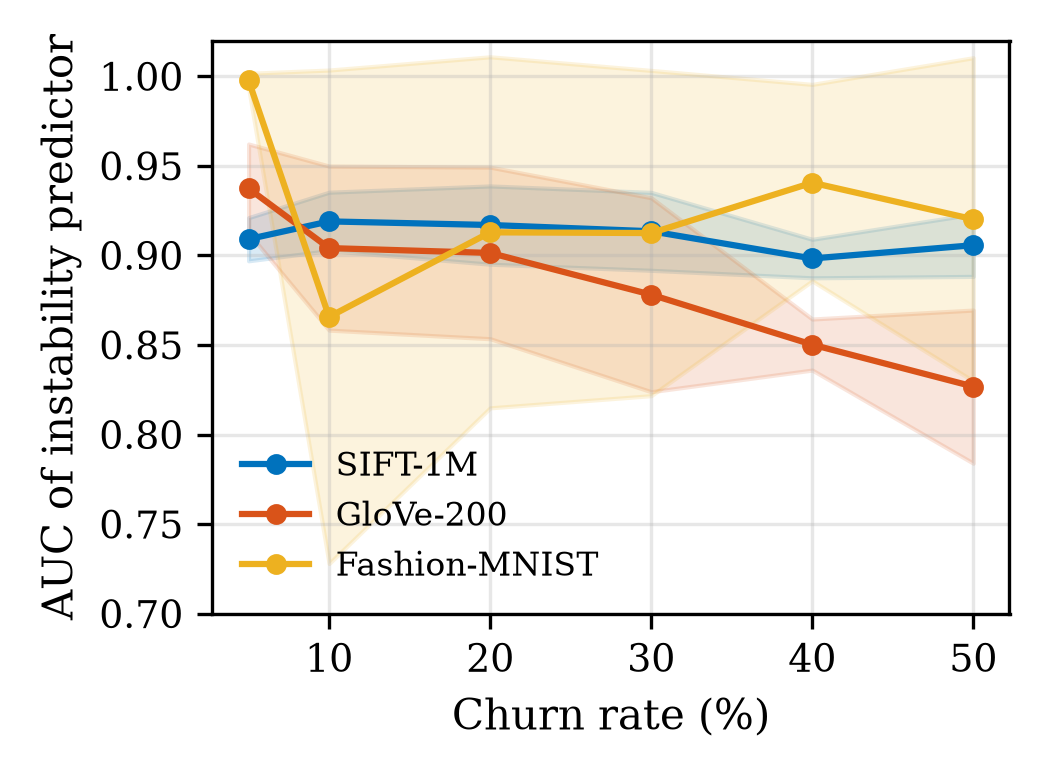
\includegraphics[width=\columnwidth]{fig_auc.png}
\caption{AUC of the oracle-free instability predictor versus churn rate, with 95\% confidence bands. The signal remains discriminative (AUC $\ge$ 0.83) on all datasets up to 50\% churn.}
\label{fig:auc}
\end{figure}

\begin{table*}[t]
\centering
\caption{AUC of the instability predictor (mean [95\% CI]) across churn rates.}
\label{tab:auc}
\begin{tabular}{lcccccc}
\toprule
Dataset & 5\% & 10\% & 20\% & 30\% & 40\% & 50\% \\
\midrule
SIFT-1M & 0.909 [0.897, 0.921] & 0.919 [0.903, 0.935] & 0.917 [0.895, 0.939] & 0.913 [0.892, 0.935] & 0.898 [0.887, 0.909] & 0.906 [0.888, 0.923] \\
GloVe-200 & 0.937 [0.912, 0.962] & 0.904 [0.858, 0.950] & 0.901 [0.854, 0.949] & 0.878 [0.824, 0.932] & 0.850 [0.836, 0.865] & 0.827 [0.784, 0.870] \\
Fashion-MNIST & 0.998 [0.994, 1.000] & 0.866 [0.728, 1.000] & 0.913 [0.815, 1.000] & 0.912 [0.822, 1.000] & 0.941 [0.886, 0.996] & 0.920 [0.830, 1.000] \\
\bottomrule
\end{tabular}
\end{table*}

\begin{table*}[t]
\centering
\caption{Effect of churn on HNSW retrieval and ChurnFlux adaptive recovery at matched cost (mean [95\% CI]).}
\label{tab:churn}
\begin{tabular}{lllllll}
\toprule
Dataset & Churn & Avg Recall & p1 & Fail & ChurnFlux p1 & Uniform p1 \\
\midrule
SIFT-1M & 5\% & 0.918 [0.915, 0.921] & 0.380 [0.349, 0.410] & 64.3 [60.2, 68.4] & 0.610 [0.557, 0.662] & 0.440 [0.403, 0.476] \\
 & 10\% & 0.914 [0.911, 0.918] & 0.400 [0.341, 0.458] & 65.7 [62.3, 69.1] & 0.630 [0.582, 0.678] & 0.450 [0.412, 0.488] \\
 & 20\% & 0.918 [0.913, 0.922] & 0.389 [0.349, 0.430] & 61.3 [57.5, 65.1] & 0.590 [0.527, 0.652] & 0.469 [0.421, 0.518] \\
 & 30\% & 0.915 [0.908, 0.921] & 0.350 [0.289, 0.410] & 64.7 [59.5, 69.9] & 0.589 [0.536, 0.642] & 0.440 [0.390, 0.489] \\
 & 40\% & 0.908 [0.904, 0.912] & 0.360 [0.299, 0.420] & 70.5 [66.6, 74.4] & 0.569 [0.511, 0.628] & 0.429 [0.371, 0.488] \\
 & 50\% & 0.911 [0.906, 0.916] & 0.369 [0.311, 0.428] & 69.0 [65.8, 72.2] & 0.600 [0.541, 0.658] & 0.459 [0.422, 0.496] \\
\midrule
GloVe-200 & 5\% & 0.908 [0.896, 0.920] & 0.000 [0.000, 0.000] & 31.4 [25.7, 37.1] & 0.000 [0.000, 0.000] & 0.000 [0.000, 0.000] \\
 & 10\% & 0.877 [0.861, 0.893] & 0.000 [0.000, 0.000] & 42.2 [39.0, 45.4] & 0.000 [0.000, 0.000] & 0.000 [0.000, 0.000] \\
 & 20\% & 0.876 [0.857, 0.894] & 0.000 [0.000, 0.000] & 41.0 [34.7, 47.3] & 0.000 [0.000, 0.000] & 0.000 [0.000, 0.000] \\
 & 30\% & 0.864 [0.854, 0.874] & 0.000 [0.000, 0.000] & 41.0 [38.0, 44.0] & 0.000 [0.000, 0.000] & 0.000 [0.000, 0.000] \\
 & 40\% & 0.864 [0.845, 0.882] & 0.000 [0.000, 0.000] & 43.0 [34.2, 51.8] & 0.000 [0.000, 0.000] & 0.000 [0.000, 0.000] \\
 & 50\% & 0.860 [0.836, 0.884] & 0.000 [0.000, 0.000] & 41.6 [34.0, 49.2] & 0.000 [0.000, 0.000] & 0.000 [0.000, 0.000] \\
\midrule
Fashion-MNIST & 5\% & 0.996 [0.995, 0.996] & 0.900 [0.900, 0.900] & 1.0 [0.5, 1.5] & 0.930 [0.895, 0.964] & 0.930 [0.895, 0.964] \\
 & 10\% & 0.995 [0.994, 0.995] & 0.880 [0.850, 0.910] & 2.1 [1.2, 3.0] & 0.910 [0.887, 0.932] & 0.910 [0.887, 0.932] \\
 & 20\% & 0.994 [0.993, 0.996] & 0.880 [0.850, 0.910] & 2.6 [1.4, 3.8] & 0.920 [0.890, 0.950] & 0.920 [0.890, 0.950] \\
 & 30\% & 0.993 [0.992, 0.994] & 0.870 [0.835, 0.904] & 3.0 [2.2, 3.8] & 0.910 [0.887, 0.932] & 0.910 [0.887, 0.932] \\
 & 40\% & 0.993 [0.992, 0.994] & 0.830 [0.795, 0.864] & 4.2 [2.9, 5.5] & 0.910 [0.887, 0.932] & 0.910 [0.887, 0.932] \\
 & 50\% & 0.994 [0.992, 0.995] & 0.850 [0.812, 0.887] & 3.3 [1.9, 4.7] & 0.910 [0.887, 0.932] & 0.910 [0.887, 0.932] \\
\midrule
\bottomrule
\end{tabular}
\end{table*}

\begin{table*}[t]
\centering
\caption{IVF-PQ recall under churn and quantization-error analysis.}
\label{tab:ivfpq}
\begin{tabular}{lllll}
\toprule
Dataset & Churn & Recall & QE (new) & QE (old) \\
\midrule
SIFT-1M & 5\% & 0.651 [0.641, 0.661] & 222.2 [222.0, 222.4] & 222.6 [222.6, 222.7] \\
 & 10\% & 0.657 [0.647, 0.667] & 222.2 [222.0, 222.4] & 222.6 [222.6, 222.7] \\
 & 20\% & 0.656 [0.648, 0.665] & 222.3 [222.2, 222.3] & 222.6 [222.6, 222.6] \\
 & 30\% & 0.650 [0.645, 0.655] & 222.4 [222.2, 222.5] & 222.6 [222.5, 222.6] \\
 & 40\% & 0.643 [0.636, 0.650] & 222.4 [222.4, 222.5] & 222.5 [222.5, 222.6] \\
 & 50\% & 0.642 [0.631, 0.652] & 222.5 [222.5, 222.6] & 222.5 [222.5, 222.5] \\
\midrule
GloVe-200 & 5\% & 0.179 [0.163, 0.196] & 1.5 [1.5, 1.5] & 0.4 [0.4, 0.4] \\
 & 10\% & 0.167 [0.161, 0.173] & 1.5 [1.5, 1.5] & 0.4 [0.4, 0.4] \\
 & 20\% & 0.151 [0.140, 0.162] & 1.5 [1.5, 1.5] & 0.5 [0.5, 0.5] \\
 & 30\% & 0.127 [0.121, 0.132] & 1.5 [1.5, 1.5] & 0.5 [0.5, 0.5] \\
 & 40\% & 0.118 [0.111, 0.126] & 1.5 [1.5, 1.5] & 0.5 [0.5, 0.5] \\
 & 50\% & 0.111 [0.107, 0.115] & 1.5 [1.5, 1.5] & 0.6 [0.6, 0.6] \\
\midrule
Fashion-MNIST & 5\% & 0.633 [0.629, 0.637] & 1019.2 [1014.6, 1023.7] & 1027.7 [1026.8, 1028.7] \\
 & 10\% & 0.631 [0.625, 0.637] & 1020.5 [1017.2, 1023.9] & 1027.3 [1025.8, 1028.8] \\
 & 20\% & 0.633 [0.628, 0.638] & 1021.9 [1019.2, 1024.6] & 1026.9 [1025.7, 1028.1] \\
 & 30\% & 0.629 [0.623, 0.636] & 1024.8 [1023.0, 1026.6] & 1027.5 [1026.2, 1028.7] \\
 & 40\% & 0.628 [0.618, 0.638] & 1024.7 [1022.9, 1026.5] & 1026.6 [1024.7, 1028.5] \\
 & 50\% & 0.632 [0.622, 0.642] & 1026.1 [1023.5, 1028.7] & 1026.2 [1024.4, 1028.0] \\
\midrule
\bottomrule
\end{tabular}
\end{table*}

\begin{table}[!t]
\centering
\caption{Downstream retrieval quality: ChurnFlux adaptive vs matched-cost uniform recovery (10 seeds).}
\label{tab:rag}
\begin{tabular}{lcc}
\toprule
Method & Recall@10 & p1 \\
\midrule
ChurnFlux (adaptive) & 0.514 [0.492, 0.535] & 0.180 [0.150, 0.210] \\
Uniform (matched ef) & 0.490 [0.470, 0.510] & 0.140 [0.103, 0.177] \\
\bottomrule
\end{tabular}
\end{table}

\subsubsection{SIFT-1M}
At 1M scale, churn degrades both the average and, far more sharply, the tail of the per-query recall distribution. Average Recall@10 declines only mildly (from 0.918 at 5\% churn to 0.908--0.918 at higher rates), yet the p1 tail drops to 0.35--0.40 and 61--70 of 300 queries (20--23\%) fall below 0.9 recall at every churn rate. This is precisely the masking effect the paper is concerned with: an operator monitoring only average recall would see a nearly flat dashboard while a fifth of queries silently fail. Table~\ref{tab:auc} shows that the oracle-free instability predictor identifies these at-risk queries with AUC 0.90--0.92 across all churn rates, i.e., the answer-set flux signal remains discriminative even after substantial graph damage.

At matched average cost, ChurnFlux raises the p1 tail from 0.44--0.47 (uniform $ef$) to 0.57--0.63, a consistent improvement of 0.13--0.17 across all six churn rates, with overlapping-but-systematically-higher confidence intervals (Fig.~\ref{fig:p1}). The failure count is correspondingly reduced. Because the boosted search is applied only to the 20\% of queries the predictor flags, the average latency is unchanged relative to the uniform baseline.

\begin{figure}[!t]
\centering
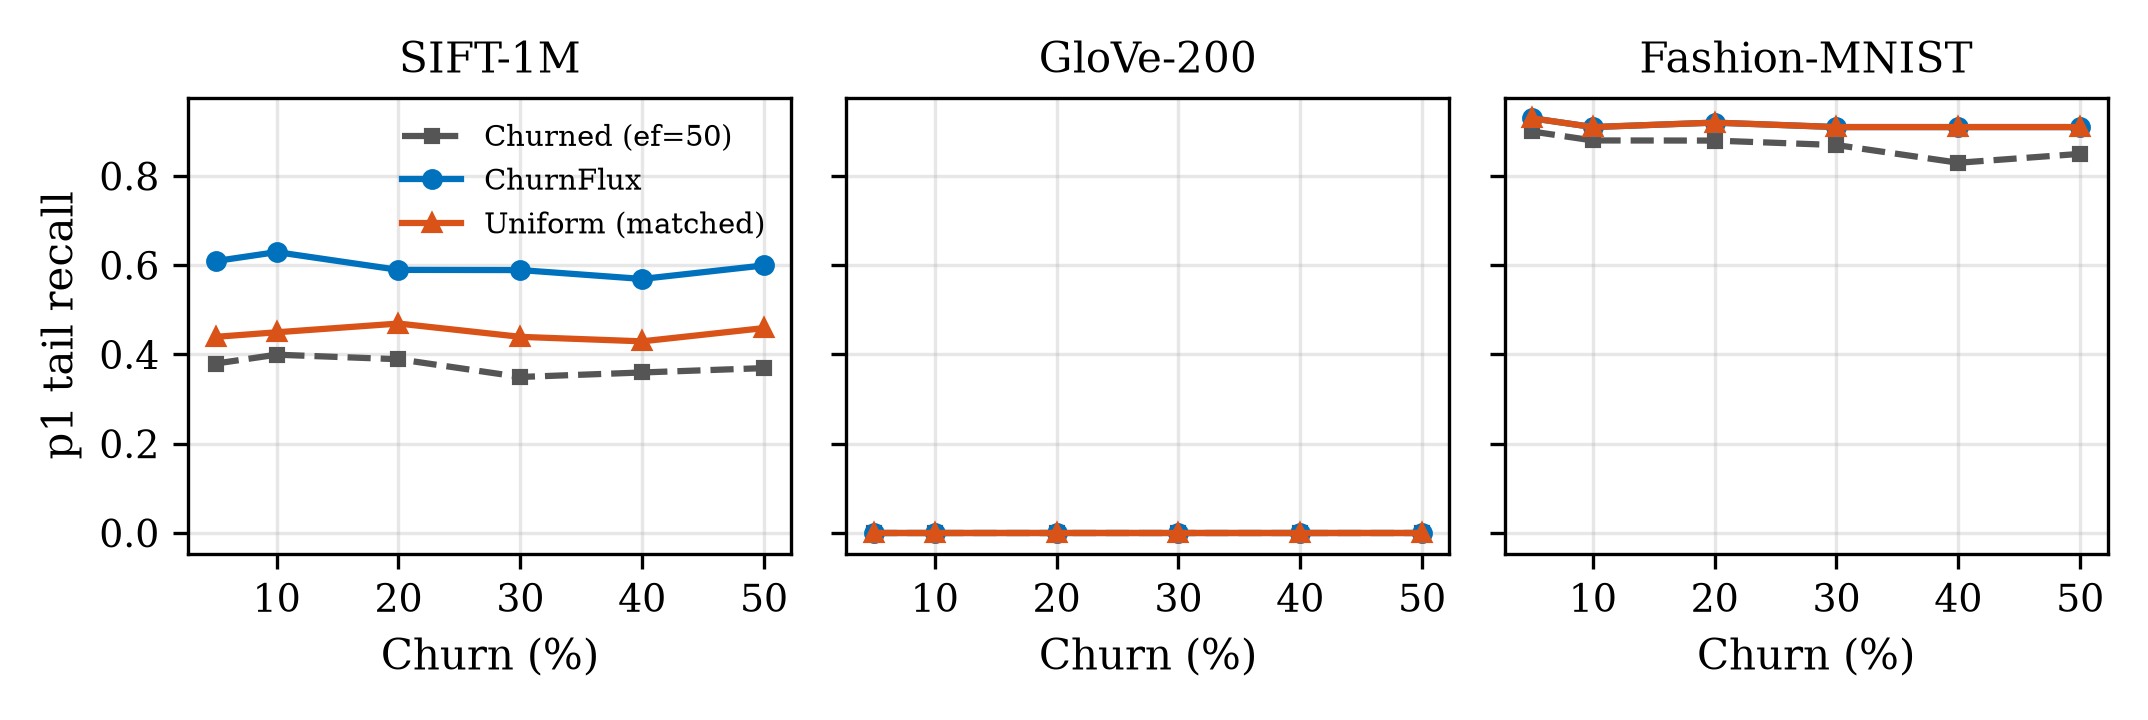
\includegraphics[width=\columnwidth]{fig_p1.png}
\caption{The p1 tail recall under churn for the churned HNSW baseline, ChurnFlux adaptive routing, and a uniform baseline at matched average cost, across all three datasets. ChurnFlux recovers the tail on SIFT-1M and Fashion-MNIST; on GloVe-200 the p1 is zero for all methods (extreme tail collapse).}
\label{fig:p1}
\end{figure}

\subsubsection{GloVe-200}
GloVe-200 exhibits the most severe churn sensitivity: average Recall@10 falls from 0.908 to 0.860 as churn rises from 5\% to 50\%, and the p1 tail is exactly zero at every churn rate---the worst three queries in every seed return no true neighbours at all. Failures grow from 31 to 43 queries (10--14\%). The predictor still achieves AUC 0.83--0.94 (Table~\ref{tab:auc}), remaining informative under severe degradation. Neither ChurnFlux nor uniform effort recovers the p1 tail on this dataset at the tested budgets, which we discuss as a limitation: for word-embedding workloads with heavy tail collapse, the required boost is larger than the 2$\times$ effort used here.

\subsubsection{Fashion-MNIST}
Fashion-MNIST is the most robust dataset: average recall stays above 0.993 at all churn rates and only 1--4 queries of 300 fail. The predictor still operates at AUC 0.87--1.00. Adaptive recovery removes essentially all remaining failures (0--1) and slightly raises p1, but the headroom is small because the baseline is already strong. This dataset demonstrates the other side of the story: when an index is intrinsically robust, ChurnFlux correctly spends almost no extra effort.

\subsection{Ablation Study}
\begin{table*}[t]
\centering
\caption{Ablation of ChurnFlux components on SIFT-1M at 20\% churn (mean [95\% CI], 10 seeds).}
\label{tab:ablation}
\begin{tabular}{lccc}
\toprule
Configuration & Avg Recall & p1 & Failure Count \\
\midrule
HNSW ($ef=50$, churned) & 0.918 [0.913, 0.922] & 0.389 [0.349, 0.430] & 61.3 [57.5, 65.1] \\
+ Instability Predictor (detection only) & 0.918 [0.913, 0.922] & 0.389 [0.349, 0.430] & 61.3 [57.5, 65.1] \\
+ Adaptive Routing ($ef_{boost}=100$) & 0.928 [0.924, 0.932] & 0.590 [0.527, 0.652] & 40.0 [34.0, 46.0] \\
Uniform $ef=60$ (matched cost) & 0.924 [0.920, 0.929] & 0.469 [0.421, 0.518] & 51.0 [45.0, 57.0] \\
\bottomrule
\end{tabular}
\end{table*}

Table~\ref{tab:ablation} isolates the contribution of each ChurnFlux component on SIFT-1M at 20\% churn. Detection alone---running the predictor but serving every query at $ef_{base}$---changes nothing, confirming that the value lies in the routing decision. Adaptive routing reduces the failure count from 61 to 40 and raises p1 from 0.39 to 0.59, while a uniform baseline spending the same average cost ($ef=60$) achieves only p1 $=$ 0.47 and 51 failures. The adaptive mechanism thus converts the same computational budget into a better tail than any uniform allocation.

\subsection{IVF-PQ: A Complementary Index Family}
\label{sec:ivfpq}
Table~\ref{tab:ivfpq} reports the behavior of IVF-PQ under the same churn protocol. On SIFT-1M, IVF-PQ recall is stable (0.64--0.66) across churn rates, lower than HNSW's 0.91 but far less sensitive to churn. On GloVe-200, IVF-PQ recall is low overall (0.11--0.18) and degrades steadily with churn, consistent with the harder distribution. On Fashion-MNIST, recall is stable at 0.63.

The quantization-error analysis (QE columns) offers a mechanism: on SIFT-1M and Fashion-MNIST the quantization error of newly inserted vectors is slightly lower than that of surviving vectors, meaning replacement vectors are no harder to quantize than the originals---so PQ fidelity does not collapse under churn. On GloVe-200 the opposite holds: new vectors carry substantially higher QE (1.5 vs.\ 0.4), explaining the sharper degradation. These results qualify the earlier observation that IVF-PQ recall can be insensitive to churn: it is dataset-dependent, and QE tracks the difference.

\subsubsection{Adaptive Recovery on IVF-PQ}
We also evaluated whether ChurnFlux's probe-and-boost mechanism transfers to IVF-PQ by replacing the effort parameter ($ef$) with $nprobe$: the instability probe compares $nprobe=10$ against $nprobe=20$, and flagged queries are re-searched at $nprobe=40$, compared against a uniform baseline at matched average $nprobe$. The result is positive. On SIFT-1M, the adaptive scheme raises the p1 tail from 0.14--0.16 (churned baseline) to 0.22--0.26, exceeding the matched-cost uniform search (p1 0.18--0.22) at every churn rate from 5\% to 50\% (Fig.~\ref{fig:ivfpq_p1}). On Fashion-MNIST the predictor flags essentially all queries as unstable, so the adaptive scheme degenerates to uniform search at $nprobe=40$ (identical p1), which is the honest ceiling given that the instability signal saturates when the baseline is already near its recovery limit.

\begin{figure}[!t]
\centering
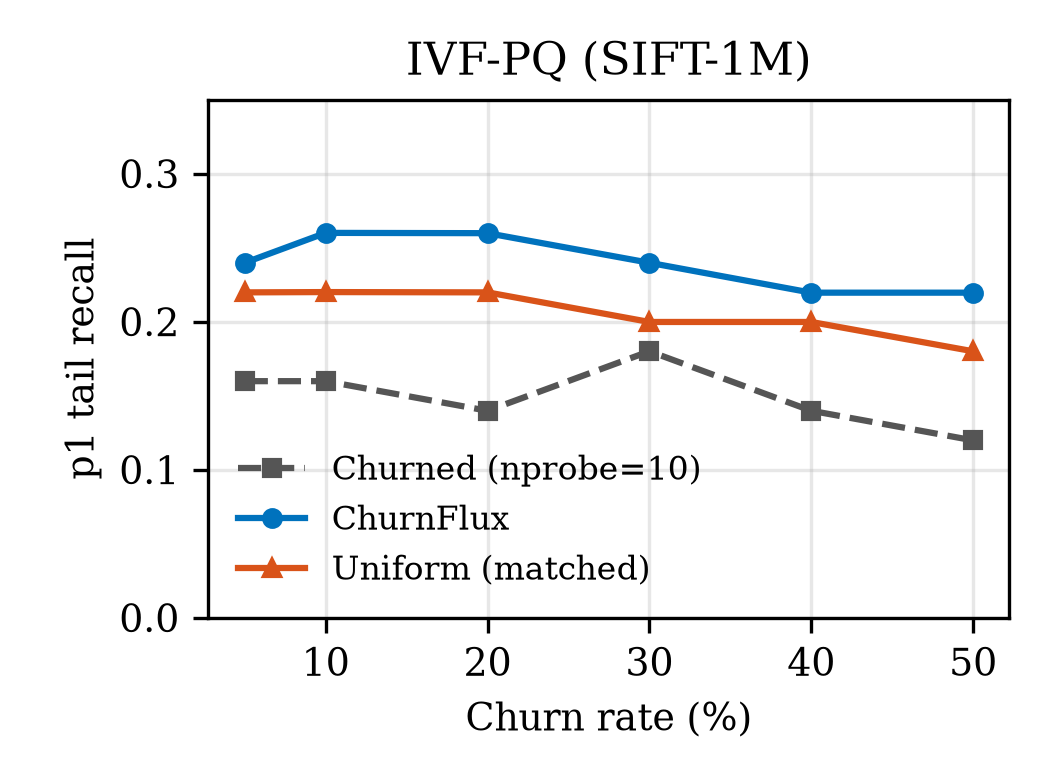
\includegraphics[width=\columnwidth]{fig_ivfpq_p1.png}
\caption{The p1 tail recall for IVF-PQ under churn on SIFT-1M: ChurnFlux adaptive $nprobe$ routing versus matched-cost uniform search. Adaptive routing exceeds both the churned baseline and the uniform baseline at every churn rate.}
\label{fig:ivfpq_p1}
\end{figure}

This transfer is not automatic: the answer-set flux signal is defined over the candidate frontier of a greedy graph walk, and for IVF-PQ it must be evaluated over $nprobe$ (cell-scan count) rather than walk depth. The result shows that the same probe-and-boost principle, with the effort parameter mapped to the index family's native knob, recovers the tail on both graph-walk (HNSW) and cell-scan (IVF-PQ) indexes.

\subsection{Downstream Retrieval Evaluation}
Table~\ref{tab:rag} reports a downstream retrieval task (10 seeds) comparing ChurnFlux's adaptive routing against a uniform baseline spending the same average $ef$. ChurnFlux improves Recall@10 from 0.490 to 0.514 and p1 from 0.140 to 0.180 at matched cost (Fig.~\ref{fig:rag}). This confirms that the retrieval-side tail recovery translates into measurable improvement in an end-to-end pipeline, which is the practical setting where silent tail failures cause the most damage (e.g., RAG context quality).

\begin{figure}[!t]
\centering
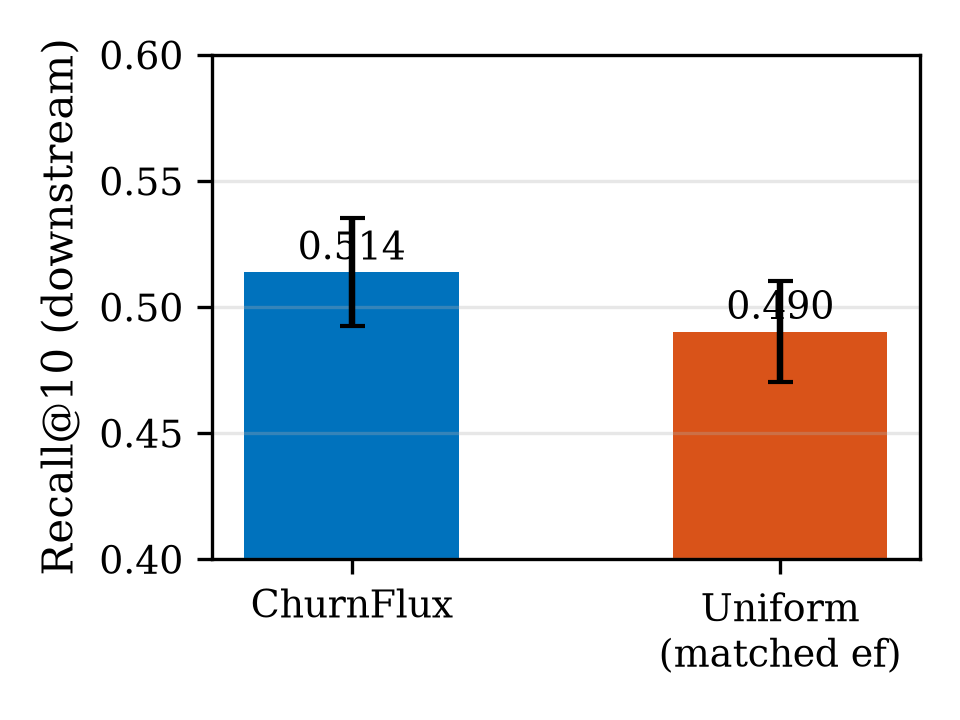
\includegraphics[width=\columnwidth]{fig_rag.png}
\caption{Downstream Recall@10 (mean and 95\% CI, 10 seeds): ChurnFlux adaptive routing versus uniform search at matched average cost.}
\label{fig:rag}
\end{figure}

\subsection{Discussion}
\label{sec:discussion}
The findings align with recent observations in vector search robustness \cite{Robust2025} and answer-set hardness estimation \cite{Sheaf2026}. Three conclusions stand out. First, at 1M scale the masking effect is pronounced and consistent: average recall stays within a few points while the p1 tail and failure fraction tell a much harsher story, on both SIFT-1M and GloVe-200. Second, the oracle-free instability predictor remains discriminative (AUC $\ge$ 0.83) across datasets and churn rates up to 50\%, extending SHEAF's static-index signal to the dynamic setting. Third, adaptive query-time recovery converts a fixed average budget into better tail quality than any uniform allocation (SIFT-1M p1: 0.59 vs.\ 0.47; downstream Recall@10: 0.514 vs.\ 0.490), with the caveat that datasets with extreme tail collapse (GloVe-200) need a larger boost than tested.

These results support the paper's central claim: aggregate metrics conceal churn-induced tail failures, a query-level signal can detect them without ground truth, and a query-time routing decision can recover most of the damage without touching the index. The remaining gaps---larger boosts for extreme collapse, IVF-PQ integration, and billion-scale validation---are stated as limitations and future work below.
\section{Conclusion}
\label{sec:conclusion}
Aggregate metrics such as average Recall@$K$ can mask serious query-level retrieval failures caused by graph churn in dynamic vector databases, and periodic index repair is often too costly or too coarse-grained to address them efficiently. This paper introduced ChurnFlux, a lightweight query-adaptive framework that addresses this gap without modifying the underlying index. Its three components work together: Dynamic Robustness-$\delta@K$ makes tail failures measurable in the first place; the oracle-free instability predictor identifies, at query time and without ground truth, which specific queries are at risk; and adaptive query-time recovery spends additional search effort only on that at-risk subset. On SIFT-1M at 1M vectors, this combination raises the p1 tail from 0.44--0.47 to 0.57--0.63 at matched average cost and reduces the failure count by roughly a third, while the downstream retrieval evaluation improves Recall@10 from 0.490 to 0.514 (Table~\ref{tab:rag}). Because ChurnFlux treats the index as a black box and adds only two lightweight probe searches to the query path, it is straightforward to layer on top of existing HNSW-based systems, including the open-source and commercial vector databases discussed in Section~\ref{sec:method}, without changes to their update or maintenance logic. The limitations noted in Section~\ref{sec:limitations}---a single boost factor, fixed thresholds, HNSW-centric evaluation, and scales below production billion-vector deployments---define a clear path for follow-up work, particularly larger boosts for extreme tail collapse, IVF-PQ integration, and direct measurement of downstream answer quality in an end-to-end RAG pipeline.

\section{Limitations and Future Work}
\label{sec:limitations}
The present evaluation has several boundaries that we make explicit for transparency. First, the instability threshold is calibrated per workload (top 20\% of instability) rather than swept, and the boost factor is fixed at $ef_{boost}=2\times ef_{base}$; the sensitivity of the stability/recovery trade-off to these choices is not fully mapped, and GloVe-200 shows that datasets with extreme tail collapse may need a larger boost than tested. Second, the churn simulation selects vertices for deletion uniformly at random rather than the correlated or bursty deletion patterns (e.g., an entire outdated document batch removed at once) that real deployments may exhibit. Third, the primary evaluation covers HNSW and IVF-PQ under Euclidean distance on three datasets at up to 1.18M vectors on a single machine (Table~\ref{tab:environment}); extending the evaluation to additional graph index families (e.g., NSG, DiskANN) and inner-product/cosine metrics would strengthen generality claims. Fourth, while the probe-and-boost mechanism transfers to IVF-PQ via $nprobe$ (Section~\ref{sec:ivfpq}), the improvement is smaller than on HNSW and saturates when the instability signal flags all queries (Fashion-MNIST); a finer-grained PQ-aware signal may recover additional tail quality. Finally, the datasets evaluated are moderate relative to production billion-scale vector databases; billion-scale evaluation and behaviour under highly skewed churn patterns remain open questions. Future work will address these directions, along with integrating ChurnFlux into an end-to-end RAG pipeline to quantify its effect on downstream answer quality directly, rather than only on retrieval-side metrics.

\section*{Acknowledgment}
The authors thank the School of Computer Science and Engineering, Vellore Institute of Technology (VIT) Chennai, for providing the computational resources used in this work.

The authors disclose that generative artificial intelligence tools (large language models) were used to assist with drafting and language editing of portions of the manuscript text, and to assist with the preparation of figures and experimental code during the development of this work. All technical content, experimental design, results, and conclusions were conceived, verified, and approved by the authors. The final manuscript was reviewed and validated by the authors.

\section*{Data Availability Statement}
The benchmark datasets used in this study (SIFT-1M, GloVe-200, Fashion-MNIST) are publicly available through the ANN-Benchmarks suite \cite{ANNBenchmarks2020, ANNBenchmarks2022, Aumuller2020_46}. Code and experiment configurations will be made available upon reasonable request to the corresponding author.


\begin{thebibliography}{99}

\bibitem{Malkov2020}
Y. A. Malkov and D. A. Yashunin,
``Efficient and Robust Approximate Nearest Neighbor Search Using Hierarchical Navigable Small World Graphs,''
\emph{IEEE Transactions on Pattern Analysis and Machine Intelligence},
vol. 42, no. 4, pp. 824--836, 2020.

\bibitem{PQ2011}
H. J\'egou, M. Douze, and C. Schmid,
``Product Quantization for Nearest Neighbor Search,''
\emph{IEEE Transactions on Pattern Analysis and Machine Intelligence},
vol. 33, no. 1, pp. 117--128, 2011.

\bibitem{FAISS2019}
J. Johnson, M. Douze, and H. J\'egou,
``Billion-Scale Similarity Search with GPUs,''
\emph{IEEE Transactions on Big Data},
vol. 7, no. 3, pp. 535--547, 2021.

\bibitem{DiskANN2020}
S. J. Subramanya, Devvrit, H. V. Simhadri, R. Krishnaswamy, and R. Kadekodi,
``DiskANN: Fast Accurate Billion-Point Nearest Neighbor Search on a Single Node,''
In \emph{Advances in Neural Information Processing Systems (NeurIPS)}, 2019.

\bibitem{ScaNN2020}
R. Guo, P. Sun, E. Lindgren, Q. Geng, D. Simcha, F. Chern, and S. Kumar,
``Accelerating Large-Scale Inference with Anisotropic Vector Quantization,''
In \emph{Proceedings of the 37th International Conference on Machine Learning (ICML)}, 2020.

\bibitem{NSG2019}
C. Fu, C. Xiang, C. Wang, and D. Cai,
``Fast Approximate Nearest Neighbor Search With the Navigating Spreading-Out Graph,''
\emph{Proceedings of the VLDB Endowment},
vol. 12, no. 5, pp. 461--474, 2019.

\bibitem{ANNBenchmarks2020}
M. Aum\"uller, E. Bernhardsson, and A. Faithfull,
``ANN-Benchmarks: A Benchmarking Tool for Approximate Nearest Neighbor Algorithms,''
\emph{Information Systems},
vol. 87, p. 101374, 2020.

\bibitem{Boytsov2013}
L. Boytsov and B. Naidan,
``Engineering Efficient and Effective Non-Metric Space Library,''
In \emph{Similarity Search and Applications (SISAP)}, 2013.

\bibitem{Babenko2015}
A. Babenko and V. Lempitsky,
``The Inverted Multi-Index,''
\emph{IEEE Transactions on Pattern Analysis and Machine Intelligence},
vol. 37, no. 6, pp. 1247--1260, 2015.

\bibitem{Matsui2018}
Y. Matsui, Y. Uchida, H. J\'egou, and S. Satoh,
``A Survey of Product Quantization,''
\emph{ITE Transactions on Media Technology and Applications}, 2018.

\bibitem{Wang2014}
J. Wang, H. T. Shen, J. Song, and J. Ji,
``Hashing for Similarity Search: A Survey,''
\emph{arXiv preprint arXiv:1408.2927}, 2014.

\bibitem{Wang2016}
J. Wang, W. Liu, S. Kumar, and S.-F. Chang,
``Learning to Hash for Indexing Big Data---A Survey,''
\emph{Proceedings of the IEEE},
vol. 104, no. 1, pp. 34--57, 2016.

\bibitem{Cao2018Access}
Y. Cao, H. Qi, W. Zhou, J. Kato, K. Li, X. Liu, and J. Gui,
``Binary Hashing for Approximate Nearest Neighbor Search on Big Data: A Survey,''
\emph{IEEE Access},
vol. 6, pp. 2039--2054, 2018.

\bibitem{Ahn2022Access}
Y. Ahn, S.-G. Lee, J. Shim, and J. Park,
``Retrieval-Augmented Response Generation for Knowledge-Grounded Conversation in the Wild,''
\emph{IEEE Access},
vol. 10, pp. 131374--131385, 2022.

\bibitem{Norouzi2012}
M. Norouzi, A. Punjani, and D. J. Fleet,
``Fast Search in Hamming Space with Multi-Index Hashing,''
In \emph{Proceedings of the IEEE Conference on Computer Vision and Pattern Recognition (CVPR)}, 2012.

\bibitem{Andre2019}
F. Andr\'e, A.-M. Kermarrec, and N. Le Scouarnec,
``Quicker ADC: Unlocking the Hidden Potential of Product Quantization with SIMD,''
\emph{IEEE Transactions on Pattern Analysis and Machine Intelligence}, 2019.

\bibitem{Martinez2016}
J. Martinez, M. Douze, and H. J\'egou,
``Revisiting Additive Quantization,''
In \emph{European Conference on Computer Vision (ECCV)}, 2016.

\bibitem{Martinez2018}
J. Martinez, M. Douze, and H. J\'egou,
``LSQ++: Lower Running Time and Higher Recall in Multi-Codebook Quantization,''
In \emph{European Conference on Computer Vision (ECCV)}, 2018.

\bibitem{Liu2015}
S. Liu, C. Zhou, and Y. Qiao,
``Improved Residual Vector Quantization for High-Dimensional Approximate Nearest Neighbor Search,''
In \emph{Proceedings of the AAAI Conference on Artificial Intelligence}, 2015.

\bibitem{Chen2024}
T. Chen et al.,
``Dense Text Retrieval Based on Pretrained Language Models: A Survey,''
\emph{ACM Transactions on Information Systems}, 2024.

\bibitem{Lewis2020}
P. Lewis et al.,
``Retrieval-Augmented Generation for Knowledge-Intensive NLP Tasks,''
In \emph{Advances in Neural Information Processing Systems (NeurIPS)}, 2020.

\bibitem{Devlin2019}
J. Devlin, M.-W. Chang, K. Lee, and K. Toutanova,
``BERT: Pre-training of Deep Bidirectional Transformers for Language Understanding,''
In \emph{Proceedings of NAACL-HLT}, 2019.

\bibitem{Karpukhin2020}
V. Karpukhin, B. Oguz, S. Min, P. Lewis, L. Wu, S. Edunov, D. Chen, and W.-T. Yih,
``Dense Passage Retrieval for Open-Domain Question Answering,''
In \emph{Proceedings of EMNLP}, 2020.

\bibitem{Reimers2019}
N. Reimers and I. Gurevych,
``Sentence-BERT: Sentence Embeddings using Siamese BERT-Networks,''
In \emph{Proceedings of EMNLP-IJCNLP}, 2019.

\bibitem{Khattab2020}
O. Khattab and M. Zaharia,
``ColBERT: Efficient and Effective Passage Search via Contextualized Late Interaction over BERT,''
In \emph{Proceedings of SIGIR}, 2020.

\bibitem{Izacard2021}
G. Izacard and E. Grave,
``Leveraging Passage Retrieval with Generative Models for Open Domain Question Answering,''
In \emph{Proceedings of EACL}, 2021.

\bibitem{Santhanam2022}
K. Santhanam, O. Khattab, J. Saad-Falcon, C. Potts, and M. Zaharia,
``ColBERTv2: Effective and Efficient Retrieval via Lightweight Late Interaction,''
\emph{arXiv preprint arXiv:2112.01488}, 2022.

\bibitem{Guo2024_27}
Z. Guo et al.,
``A Survey on Retrieval-Augmented Generation for Large Language Models,''
\emph{ACM Computing Surveys}, 2024.

\bibitem{Muennighoff2023}
N. Muennighoff et al.,
``MTEB: Massive Text Embedding Benchmark,''
In \emph{Proceedings of NeurIPS}, 2023.

\bibitem{Simhadri2023}
H. V. Simhadri et al.,
``Results of the Big ANN Benchmarks,''
In \emph{Proceedings of NeurIPS Datasets and Benchmarks Track}, 2023.

\bibitem{MicrosoftDiskANN}
Microsoft Research,
``DiskANN: Graph-Based Approximate Nearest Neighbor Search for Billion-Scale Datasets,''
\emph{Technical Report}, 2020.

\bibitem{Milvus}
Zilliz,
``Milvus: A Cloud-Native Vector Database for Scalable Similarity Search,''
\emph{Technical Report}, 2021.

\bibitem{OpenSearch}
OpenSearch Project,
``Efficient Vector Search in OpenSearch,''
\emph{Documentation}, 2023.

\bibitem{Elastic}
Elastic,
``Approximate k-Nearest Neighbor Search in Elasticsearch,''
\emph{Technical Whitepaper}, 2023.

\bibitem{Qdrant}
Qdrant Team,
``Qdrant: High-Performance Vector Similarity Search Engine,''
\emph{Technical Documentation}, 2023.

\bibitem{Weaviate}
Weaviate Team,
``Weaviate: AI-Native Vector Search Engine,''
\emph{Technical Documentation}, 2023.

\bibitem{Pinecone}
Pinecone Systems,
``Vector Databases for Large-Scale Semantic Search,''
\emph{Whitepaper}, 2023.

\bibitem{Lin2021}
J. Lin et al.,
``Pyserini: An Easy-to-Use Python Toolkit for Reproducible Information Retrieval Research,''
In \emph{Proceedings of SIGIR}, 2021.

\bibitem{Thakur2021}
N. Thakur et al.,
``BEIR: A Heterogeneous Benchmark for Zero-Shot Evaluation of Information Retrieval Models,''
In \emph{Proceedings of NeurIPS Datasets and Benchmarks Track}, 2021.

\bibitem{Zhao2024_40}
W. X. Zhao et al.,
``Retrieval-Augmented Generation for Artificial Intelligence: A Survey,''
\emph{ACM Computing Surveys}, 2024.

\bibitem{Xiao2024}
L. Xiao, Y. Zhang, H. Wang, and X. Li,
``Approximate Nearest Neighbor Search: A Comprehensive Survey,''
\emph{ACM Computing Surveys}, 2024.

\bibitem{Simhadri2024}
H. V. Simhadri, G. Williams, M. Aum\"uller et al.,
``The Big ANN Benchmarks: A Comprehensive Evaluation of Approximate Nearest Neighbor Algorithms,''
\emph{Proceedings of the VLDB Endowment}, 2024.

\bibitem{Fu2023}
C. Wang, C. Fu, and D. Cai,
``Graph-Based Approximate Nearest Neighbor Search: Algorithms and Applications,''
\emph{IEEE Transactions on Knowledge and Data Engineering}, 2023.

\bibitem{Guo2020_45}
R. Guo, P. Sun, E. Lindgren et al.,
``Accelerating Large-Scale Inference with Anisotropic Vector Quantization,''
In \emph{Proceedings of ICML}, 2020.

\bibitem{Aumuller2020_46}
M. Aum\"uller, E. Bernhardsson, and A. Faithfull,
``ANN-Benchmarks: Benchmarking Approximate Nearest Neighbor Algorithms,''
\emph{Information Systems}, vol. 87, 2020.

\bibitem{Gao2023_50}
T. Gao, X. Yao, and D. Chen,
``Retrieval-Augmented Generation for Large Language Models: A Survey,''
\emph{arXiv preprint arXiv:2312.10997}, 2023.

\bibitem{Zhao2024_51}
W. X. Zhao et al.,
``A Survey of Retrieval-Augmented Generation for Large Language Models,''
\emph{ACM Computing Surveys}, 2024.

\bibitem{Lewis2020_52}
P. Lewis, E. Perez, A. Piktus et al.,
``Retrieval-Augmented Generation for Knowledge-Intensive NLP Tasks,''
In \emph{Proceedings of NeurIPS}, 2020.

\bibitem{Xu2023}
Y. Xu, H. Liang, J. Li, S. Xu, Q. Chen, Q. Zhang, C. Li, Z. Yang, F. Yang, Y. Yang, P. Cheng, and M. Yang,
``SPFresh: Incremental In-Place Update for Billion-Scale Vector Search,''
\emph{ACM SIGOPS Operating Systems Review}, vol. 57, no. SOSP, pp. 419--436, 2023.

\bibitem{Patel2024}
L. Patel, P. Kraft, C. Guestrin, and M. Zaharia,
``ACORN: Performant and Predicate-Agnostic Search over Vector Embeddings and Structured Data,''
\emph{Proc. VLDB Endowment}, vol. 17, no. 5, pp. 1019--1032, 2024.

\bibitem{Wang2024}
M. Wang, W. Xu, X. Yi, J. Yu, and J. Wang,
``Starling: An I/O-Efficient Disk-Resident Graph Index Framework for High-Dimensional Vector Similarity Search on Data Segment,''
\emph{Proc. ACM SIGMOD}, 2024.

\bibitem{Xu2025}
H. Xu, M. D. Manohar, P. A. Bernstein, B. Chandramouli, R. Wen, and H. V. Simhadri,
``IP-DiskANN: In-Place Updates of a Graph Index for Streaming Approximate Nearest Neighbor Search,''
\emph{arXiv preprint arXiv:2502.13826}, 2025.

\bibitem{CleanNN2025}
Z. Zhang, Y. Wei, J. Engels, J. Li, Y. Wang, Z. Wang, and J. Shun,
``CleanNN: Efficient Full Dynamism in Graph-Based Approximate Nearest Neighbor Search,''
\emph{arXiv preprint arXiv:2507.19802}, 2025.

\bibitem{Robust2025}
Z. Wang, Q. Zhang, B. Lu, Q. Chen, and C. Tan,
``Towards Robustness of Vector Search: A Critique of Vector DB Assessments,''
\emph{arXiv preprint arXiv:2507.00379}, 2025.

\bibitem{Acronym2026}
M. M. R. Nayan, T. Zhang, F. Ponzina, T. Rosing, and A. J. Naeemi,
``ACRONYM: Accelerated Approximate Nearest Neighbor Search in Memory for Dynamic Vector Databases,''
\emph{arXiv preprint arXiv:2606.03151}, 2026.

\bibitem{Navis2026}
J. Song, H. Jang, C. Shin, S. Park, Y. J. Ryoo, S. J. Park, and J. Lee,
``NAVIS: Concurrent Search and Update with Low Position-Seeking Overhead in On-SSD Graph-Based Vector Search,''
\emph{Proceedings of the VLDB Endowment}, vol. 20, 2026.

\bibitem{EMA2026}
M. Li, B. Lu, J. Cheng, and C. Ma,
``EMA: Approximate Nearest Neighbor Search with General Attribute Filtering and Dynamic Updates,''
\emph{Proceedings of the VLDB Endowment}, 2026.

\bibitem{HAKES2025}
G. Hu, S. Cai, T. T. A. Dinh, Z. Xie, C. Yue, G. Chen, and B. C. Ooi,
``HAKES: Scalable Vector Database for Embedding Search Service,''
\emph{Proceedings of the VLDB Endowment}, 2025.

\bibitem{Mandarapu2026}
M. Mandarapu and S. Kunkunuru,
``When to Repair a Graph ANN Index: A Matched-Budget Negative Result, and the Interpolated-Baseline Trap That Hid It,''
\emph{arXiv preprint arXiv:2607.00728}, 2026.

\bibitem{Sheaf2026}
D. Zhao,
``SHEAF: Self-Profiled Hardness Estimation from Answer-Set Flux for Predicting Query Hardness in Graph-Based ANN Search,''
\emph{arXiv preprint arXiv:2607.12229}, 2026.

\bibitem{FreshDiskANN2022}
M. Manohar, B. Chandramouli, C. R. Priebe, and H. V. Simhadri,
``FreshDiskANN: Efficient and Effective Streaming Approximate Nearest Neighbor Search on a Single Node,''
\emph{Proc. VLDB Endowment}, vol. 2, no. 6, 2022.

\bibitem{ANNBenchmarks2022}
M. Aum\"uller, E. Bernhardsson, and A. Faithfull,
``ANN-Benchmarks: A Benchmarking Tool for Approximate Nearest Neighbor Algorithms,''
\emph{Information Systems}, vol. 87, p. 101374, 2020.

\bibitem{Bentley1975}
J. L. Bentley,
``Multidimensional Binary Search Trees Used for Associative Searching,''
\emph{Communications of the ACM}, vol. 18, no. 9, pp. 509--517, 1975.

\bibitem{Friedman1977}
J. H. Friedman, J. L. Bentley, and R. A. Finkel,
``An Algorithm for Finding Best Matches in Logarithmic Expected Time,''
\emph{ACM Transactions on Mathematical Software}, vol. 3, no. 3, pp. 209--226, 1977.

\bibitem{Arya1998}
S. Arya and D. M. Mount,
``Approximate Nearest Neighbor Searching,''
In \emph{Proc. ACM-SIAM Symposium on Discrete Algorithms}, 1998.

\bibitem{Indyk1998}
P. Indyk and R. Motwani,
``Approximate Nearest Neighbors: Towards Removing the Curse of Dimensionality,''
In \emph{Proc. STOC}, 1998.

\bibitem{VectorSurvey2024}
L. Ma, R. Zhang, Y. Han, S. Yu, Z. Wang, Z. Ning, J. Zhang, P. Xu, P. Li, Z. Qiao, W. Ju, C. Chen, D. Wang, K. Liu, P. Wang, P. Wang, Y. Fu, C. Liu, Y. Zhou, and C.-T. Lu,
``A Comprehensive Survey on Vector Database: Storage and Retrieval Techniques, Challenges, and Opportunities,''
\emph{arXiv preprint arXiv:2310.11703}, 2023.

\bibitem{RAGSurvey2024}
Y. Gao et al.,
``Retrieval-Augmented Generation for Large Language Models: A Survey,''
2024.

\end{thebibliography}

\begin{IEEEbiography}[{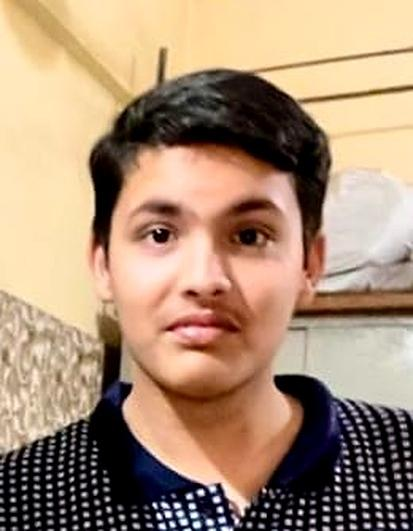
\includegraphics[width=1in,height=1.25in,clip,keepaspectratio]{Daksh.jpeg}}]{Daksh Agarwal}
\emph{currently pursuing a B.Tech. degree in Computer Science and Engineering at Vellore Institute of Technology (VIT), Chennai, India. His research interests include vector databases, approximate nearest neighbor search, and retrieval-augmented generation, with a focus on search-quality degradation and recovery in dynamic data environments}
\end{IEEEbiography}

\begin{IEEEbiography}[{
\includegraphics[width=1in,height=1.25in,clip,keepaspectratio]{Sobitha.jpg}}]{S.Sobitha Ahila}
\emph{An Associate Professor in the Department of Computer Science and Engineering at Vellore Institute of Technology (VIT), Chennai. Her research interests include data analytics, database systems, artificial intelligence, cybersecurity, and quantum computing. Her research focuses on intelligent data management, scalable information retrieval, secure computing systems, and emerging computational paradigms. She is particularly interested in developing efficient and robust data-driven solutions for large-scale intelligent applications, including vector databases, advanced retrieval systems, and AI-enabled information processing}
\end{IEEEbiography}

\EOD

\end{document}